%%%%%%%% Paper skeleton -- MLSys research track (2025 style file) %%%%%%%%%%%%%%
%
% STATUS: draft on the final kernel results (3,257 runs, R1-R6 of GAWWY_HANDOFF_PAPER.md
% folded in 2026-10-14: sampled scores and heavier models on 74 streams at 10%, R3 rerun,
% LeCaR in the kernel, native timing with the page-table walk, break-even tables). D2 is decided
% (GAWWY_HANDOFF_PAPER.md, "D2 decided"): the claim, the title, no system name, MLSys
% 2027 research track. The guard was dropped by the collaborator: do not reintroduce it.
% Numbers come from report/week_16_update, report/week_15_update and
% report/results2; each typed number carries a "% src:" comment. Nothing here is a
% new measurement. See paper-state.md and outline.md.
%
% ONE FILE: every section is in this file (search for "% ----- "). The only
% external inputs are references.bib and the generated tables in
% ../week_16_update/tables (\wsixteen), which tools/ml2/report_w16.py rewrites --
% keep those as \input so the numbers stay generated.
%
% Build:  latexmk -pdf main.tex      (MiKTeX or TeX Live)
% Check:  python <skill>/scripts/check_draft.py main.tex
%
% Colour key in the PDF:
%   red    [TODO: ...]  a missing number, experiment or decision
%   blue   [Plan: ...]  what the paragraph must say; delete when drafted
%   boxed  figure placeholders, with the data source and status
%
\documentclass{article}

\usepackage{microtype}
\usepackage{graphicx}
\usepackage{subfigure}
\usepackage{booktabs}
\usepackage{multirow}
\usepackage{array}
\usepackage{amsmath}
\usepackage{hyperref}

\newcommand{\theHalgorithm}{\arabic{algorithm}}

% Initial blind version for review:
\usepackage{mlsys2025}
% Camera-ready (only after acceptance):
% \usepackage[accepted]{mlsys2025}

\usepackage{xcolor}
\usepackage{xspace}
\usepackage{enumitem}   % compact research-question list (\S2.5)
\usepackage{pgfplots}
\pgfplotsset{compat=1.17}
\usetikzlibrary{arrows.meta,positioning,calc}
% Figure colours: the dataviz reference palette, slots 1-2 (validated colour-blind safe on
% white, all pairs) and its neutral inks. Learned linear score = blue, heavier models =
% orange, classical policies = ink. Diverging maps: blue <-> red through a gray midpoint.
\definecolor{cLin}{HTML}{2A78D6}
\definecolor{cHeavy}{HTML}{EB6834}
\definecolor{cInk}{HTML}{52514E}
\definecolor{cMuted}{HTML}{898781}
\definecolor{cGrid}{HTML}{E1E0D9}
\definecolor{cAxis}{HTML}{C3C2B7}
\definecolor{cNeg}{HTML}{E34948}
\pgfplotsset{
  paperplot/.style={
    font=\scriptsize, tick label style={font=\scriptsize}, label style={font=\scriptsize},
    axis line style={cAxis}, tick style={cAxis}, major grid style={cGrid, thin},
    every axis legend/.append style={draw=none, fill=none, font=\scriptsize},
    legend cell align=left, /tikz/every mark/.append style={solid}},
  diverging/.style={colormap={div}{rgb255=(42,120,214) rgb255=(240,239,236) rgb255=(227,73,72)}},
}
\newcommand{\figdata}{figures/data}   % written by make_figdata.py from ../results2
%==============================================================================
% ----- MACROS -----
%==============================================================================
% ---- names (one name per component, used everywhere) -----------------------
% No system name (D2, the collaborator's language rule): write "the learned policy" or
% "the linear score". ARC, LHD and S3-FIFO are always the accessed-bit forms (\S4).
\newcommand{\xv}{xv6-riscv\xspace}
\newcommand{\clock}{Clock\xspace}
\newcommand{\belady}{Belady\xspace}

% feature tiers (report/ML_REPORT.md section 4)
\newcommand{\tierF}{\textsf{F}\xspace}     % full-stream / oracle
\newcommand{\tierK}{\textsf{K}\xspace}     % kernel-observable (A/D-bit scans)
\newcommand{\tierKp}{\textsf{K+}\xspace}   % refault bookkeeping
\newcommand{\tierKKp}{\textsf{K}$\cup$\textsf{K+}\xspace}
\newcommand{\feat}[1]{\texttt{#1}}         % a single feature, e.g. \feat{idle}

% ---- generated tables from the collaborator's week-16 report (never retype) -----
% Regenerate with: cd tools/ml2 && python3 report_w15.py && python3 report_w16.py
\newcommand{\wsixteen}{../week_16_update/tables}
\newcommand{\wfifteen}{../week_15_update/tables}   % appendix dataset table only
\newcommand{\best}[1]{\textbf{#1}}   % used inside ci_main.tex: whole interval below 1

% ---- drafting marks (remove before submission; check_draft flags leftovers) --
\newcommand{\todo}[1]{\textcolor{red}{[TODO: #1]}}
\newcommand{\plan}[1]{\textcolor{blue!60!black}{\textit{[Plan: #1]}}}
\newcommand{\verify}[1]{\textcolor{orange!80!black}{[verify: #1]}}

% Figure placeholder: \figbox{height}{what it shows}{data source / status}
\newcommand{\figbox}[3]{%
  \fbox{\parbox[c][#1][c]{0.94\linewidth}{\centering\small
    \textbf{Planned figure.} #2\\[3pt]
    \textcolor{blue!60!black}{\footnotesize Source/status: #3}}}}
\newcommand{\figboxwide}[3]{%
  \fbox{\parbox[c][#1][c]{0.96\textwidth}{\centering\small
    \textbf{Planned figure.} #2\\[3pt]
    \textcolor{blue!60!black}{\footnotesize Source/status: #3}}}}

% Bold run-in finding heads (skill style rule)
\newcommand{\finding}[1]{\textbf{#1}\hspace{0.4em}}
\newcommand{\obs}[2]{\textbf{Observation #1: #2}\hspace{0.4em}}

% Draft toggle: the appendix is a SEPARATE upload at submission time.
% Keep true while drafting. For submission:
%   paper PDF:    set \withappendixfalse, build.
%   appendix PDF: set \withappendixtrue, build, keep only the pages after the
%                 references, e.g.  qpdf main.pdf --pages . <first-appendix-page>-z -- appendix.pdf
\newif\ifwithappendix
\withappendixtrue

\graphicspath{{figures/}{../figures2/}}

\mlsystitlerunning{Learned Page Replacement from What the Kernel Already Sees}

\begin{document}

\twocolumn[
% Title decided in D2 (2026-10-12).
\mlsystitle{Learned Page Replacement from What the Kernel Already Sees}

% Double-blind: the style hides authors unless [accepted]. Keep placeholders
% here anyway so a stray build never leaks names.
% Camera-ready (D2): two authors with equal contribution; legal names, affiliations
% and e-mails come from the collaborator. Mark both names with an asterisk and pass
% \mlsysEqualContribution to \printAffiliationsAndNotice. Whether the supervisor
% is an author must be settled before submissions open (19 Oct).
\begin{mlsysauthorlist}
\mlsysauthor{Anonymous Author 1}{anon}
\mlsysauthor{Anonymous Author 2}{anon}
\end{mlsysauthorlist}
\mlsysaffiliation{anon}{Anonymous Institution}
% Required by the style (without it the PDF prints "AUTHORERR"). In blind mode the
% style prints an anonymous placeholder instead; put the real one in for camera-ready.
\mlsyscorrespondingauthor{Anonymous Author 1}{anonymous@anonymous.invalid}

\mlsyskeywords{Machine Learning for Systems, Operating Systems, Page Replacement, Learned Policies}

\vskip 0.3in

\begin{abstract}
%==============================================================================
% ----- ABSTRACT -----
%==============================================================================
% Abstract: 150-220 words (median 180). Sentence roles, in order: context; problem
% and stakes; why current approaches fail; "we present"; key idea; techniques;
% evaluation basis; headline numbers WITH baseline; code.
% Every number below must appear identically in the body (paper-state.md, "Numbers").
%
% CLAIM: decided in D2 (GAWWY_HANDOFF_PAPER.md, "D2 decided", 2026-10-12). Never write
% "beats ARC". Numbers: week-16 kernel results after round 5 (74 streams at every size).
% R1/R2/R4 (2026-10-14), ci_main.tex at 10%: LeCaR vs Clock 1.113 [1.04, 1.23]; CNN / MLP /
% set-attention vs linear 1.000 / 0.998 / 0.992 (cost 87x / 150x / 79x, cost.tex); boosted
% trees 1.061 [1.01, 1.12], ranking trees 1.476 [1.05, 2.43] (worse); 32 sampled vs full
% linear 0.998 [0.97, 1.02]. 3,257 runs = rows of kernel_eval_all.csv, all "ok".
Learned policies beat hand-written heuristics in CPU caches and content-delivery
networks, but an operating system's page-replacement policy works under constraints
those settings lack: the kernel never sees individual memory accesses, cannot use
floating point on the eviction path, and every eviction changes all later faults.
We ask whether a learned page-replacement policy can work under these constraints,
and build one in the xv6 teaching kernel. It scores resident pages with a small linear
model over signals the kernel already keeps (accessed- and dirty-bit history and
refault bookkeeping), computed in whole numbers and trained offline to imitate
\belady's optimal policy.
Across 14 workloads, eight of them never used in training, and 3,257 kernel runs at
three memory sizes, the linear score incurs 8.6\% fewer page faults than \clock at 10\%
memory (95\% interval 2--15\%) and is level with ARC, the strongest classical policy we
could run in the kernel; LeCaR, a learned cache policy run in the same form, incurs 11\%
more. Five heavier models, among them a CNN and an MLP, do no better at
20--150$\times$ its cost per eviction.
Choosing a victim costs 22,803 instructions, 55$\times$ \clock; scoring 32 sampled
candidates halves that with no measurable loss. With the devices and the core we measured,
the saved faults pay for this work on a hard disk, and on an NVMe SSD with a fast core.
\todo{anonymized code link}
\end{abstract}
]

\printAffiliationsAndNotice{}

%==============================================================================
% ----- 1 INTRODUCTION -----
%==============================================================================
% =============================================================================
\section{Introduction}
\label{sec:intro}
% Budget: 1.5 pages, 1,000-1,150 words. Draft LAST among the core sections (Step 5.5).
% Moves: stakes -> today's policy and its measured failure -> why prior learned
% work does not apply -> insight (one sentence) -> challenges->techniques ->
% contributions (3-4 bullets with sections) -> headline results -> roadmap.
% Framing and claim: PENDING decision D2 (AUSTRA_HANDOFF.md, START HERE section 1).
% Do not write "beats ARC". Plain words (collaborator's language rule).
% =============================================================================

% --- Page-1 teaser ------------------------------------------------------------
% Defined at the very top of the section so it floats onto page 1.
\begin{table}[t]
\caption{\textbf{Measured in the xv6 kernel.} Page faults relative to \clock (geometric
mean over each workload's streams, then over 14 workloads with equal weight) at memory
limits of 5, 10 and 20\% of each program's pages (74 streams at each size), and
instructions spent choosing one victim among 68 candidates. Bold: the 95\% interval lies
entirely below 1. $^\dagger$Accessed-bit form: accessed bits are read at each eviction
(\S\ref{sec:impl}); LeCaR, a learned cache policy, ran at 10\% only. The learned score
beats \clock at 10\% and is level with ARC; it costs the most to decide.}
\label{tab:teaser}
\vskip 0.1in
\begin{center}
\begin{small}
\setlength{\tabcolsep}{3pt}
\begin{tabular}{@{}lrrrr@{}}
\toprule
Policy & 5\% & 10\% & 20\% & instr./victim \\
\midrule
FIFO                 & 1.23  & 1.25  & 1.35  & 385 \\
Aging                & 1.04  & 1.07  & 1.17  & 8,125 \\
LFU                  & 1.07  & 1.13  & 1.27  & 8,005 \\
\clock               & 1.00  & 1.00  & 1.00  & 411 \\
LeCaR$^\dagger$      & --    & 1.113 & --    & 8,155 \\
S3-FIFO$^\dagger$    & 1.086 & 1.016 & 1.086 & 1,395 \\
LHD$^\dagger$        & 1.005 & 0.951 & 0.949 & 14,199 \\
ARC$^\dagger$        & \textbf{0.947} & \textbf{0.943} & 0.984 & 11,934 \\
\midrule
Linear score (ours)  & 0.976 & \textbf{0.914} & 0.882 & 22,803 \\
\bottomrule
\end{tabular}
\end{small}
\end{center}
\vskip -0.1in
\end{table}
% src: report/week_16_update/tables/ci_main.tex (ARC, LHD, S3-FIFO, linear; 3 decimals;
% regenerated 2026-10-12 after round 5 / N1, 74 streams at every size)
% src: kmain_A_005/01/02 "mean" column (FIFO, Aging, LFU; 2 decimals as generated)
% src: tables/cost.tex (cost_grid.csv; QEMU instruction-count mode, 68 candidates)
% src: LeCaR row: ci_main.tex "LeCaR against Clock" (R4, 74 streams, 10% only), cost.tex
% All FINAL per AUSTRA_HANDOFF.md START HERE sections 0 and 3.

% --- Move 1: stakes --------------------------------------------------------
When a program needs more memory than it is allowed, each page fault turns a memory
access into a device access: a 4\,KB read takes 63\,\textmu s on the NVMe SSD and
8.9\,ms on the hard disk we measured (\S\ref{sec:eval-cost}). Which page the kernel
evicts decides how many of these accesses a program pays for.
% src: report/results2/device_latency.csv (S1; median 4 KB random read, no file cache)

% --- Move 2: how the OS does it today, and the measured failure --------------
The kernel must choose the page without knowing the program's future accesses. It
decides with recency heuristics built on the hardware accessed bit: \clock and its
descendants~\citep{corbato1968paging,carr1981wsclock}, and in Linux the active/inactive
lists and the multi-generational LRU~\citep{linux_mglru}. These heuristics leave many
avoidable faults. On B-tree, key-value and graph workloads, \belady's offline
policy~\citep{belady1966study} incurs 43--54\% fewer faults than \clock, and \clock is
within 2\% of exact LRU on five of the six training workloads (\S\ref{sec:bg-headroom}).
Stronger classical policies such as ARC~\citep{megiddo2003arc},
LHD~\citep{beckmann2018lhd} and S3-FIFO~\citep{yang2023s3fifo} were designed for caches
that see every hit; in the accessed-bit form a kernel can run, the best of them, ARC,
incurs about 5\% fewer faults than \clock at the two smaller memory sizes
(Table~\ref{tab:teaser}).
% src: classical tables (unchanged by the week-15 refit): Belady test 0.550 / 0.571 / 0.456 vs Clock (btree, kv, graph)
% src: week_16 tables/model_comparison.tex LRU column: 0.981-1.012 on btree, graph, kv, lzw, sort; matmul 0.879

% --- Move 3: why prior learned approaches do not solve it --------------------
Learned replacement policies outperform hand-written ones, but where every access is
visible. Hardware cache policies learn from \belady's past decisions, with the program
counter of each access as the main feature~\citep{jain2016hawkeye,shi2019glider,shah2022mockingjay}.
Content-delivery and storage caches learn from every request, in floating point, outside
the kernel~\citep{song2020lrb,song2023halp,vietri2018lecar,rodriguez2021cacheus}; even
there, three FIFO queues match the learned LRB on the traces where both were
compared~\citep{yang2023s3fifo}. A kernel has none of this visibility: it learns about a
page only when the page faults or when a scan finds its accessed or dirty bit set, and it
must pick a victim on the fault path without floating point. Learning in memory management
has so far placed pages across memory tiers~\citep{doudali2019kleio,ramaswamy2026xtier} or
tuned the parameters of far-memory reclaim~\citep{lagarcavilla2019farmemory} rather than
chosen victims. The
closest eviction work, LearnedCache~\citep{qi2026learnedcache}, runs a perceptron in the
Linux page cache through cache\_ext~\citep{zussman2025cacheext}, where every access is
visible and the pages are file pages. Learned operating-system policies at MLSys work above
the kernel~\citep{barbalho2023vmalloc,ling2025lava,zhao2026catur,yang2025byom}. We found no
learned eviction policy for a program's own memory, its anonymous pages and swap, and none
that learns only from the coarse signals a kernel has.
% src: related-work-notes.md (search of OS/arch/ML venues, 2026-10-12) and the literature
% review ML_Page_Replacement_Literature_Review.pdf (2026-10-12): "Anonymous memory and swap:
% open gap, no learned eviction policy found"; LearnedCache is page cache only. Not a
% "first" claim. S3-FIFO vs LRB: "similar efficiency" on ten random traces (LRB was too
% slow for the 6,594-trace set), S3-FIFO paper, checked 2026-10-13. Far memory: a GP
% bandit tunes the threshold controller's parameters K and S offline (ASPLOS'19 PDF).
% Kleio: RNN page scheduling DRAM/NVM; xTier: INT8 MLP in eBPF over PEBS samples.

% --- Move 4: the question and the insight ------------------------------------
We ask whether a learned page-replacement policy can work at operating-system level:
with only the signals a kernel observes, without floating point, on the eviction path,
and without knowing which program it serves. Our answer is a qualified yes:
\textbf{the kernel already sees enough}. Accessed-bit history and the refault
bookkeeping kernels already keep carry the signal a learned policy needs; a small linear
score over them, computed in whole numbers, beats \clock inside the kernel and is level
with the strongest classical policy a kernel can run. Larger models do not pay for their
cost.

% --- Move 5: challenges -> techniques (the paper's spine; see paper-state.md) --
Five problems stand in the way, and each design element answers one. The kernel never
sees accesses, so the features come from accessed/dirty-bit scans and refault
bookkeeping (\S\ref{sec:design-features}). Training data sampled naively teaches the
policy to evict the page being streamed through, so we record eviction decisions with
the most recent pages always included and protect new pages for a few scans
(\S\ref{sec:design-train}). There is no floating point on the fault path, so the score
is a whole-number dot product (\S\ref{sec:design-int}). A wrong model can be worse than
\clock, so models are chosen on validation streams only and every victim is checked
(\S\ref{sec:design-wrong}). Scoring every page is slow, so the policy can score 32
sampled candidates instead (\S\ref{sec:design-cost}).

% --- Move 6: contributions ----------------------------------------------------
Our contributions are:
\begin{itemize}
\item \textbf{A learned page-replacement policy that runs inside a kernel}: a whole-number
  linear score over kernel-visible signals, with per-process weights and sampled
  scoring, plus five heavier models (CNN, MLP, set-attention, boosted and ranking trees)
  in whole-number form (\S\ref{sec:design}, \S\ref{sec:impl}).
\item \textbf{A study of what a learned eviction policy needs.} Oracle inputs help
  richer models by 2--5\% on the workloads they were trained on and make them fail on
  real application traces; with kernel-visible inputs, more capacity does not pay
  (\S\ref{sec:bg}, \S\ref{sec:eval-info}, \S\ref{sec:eval-ablate}).
\item \textbf{An in-kernel evaluation against strong classical policies}: 14 workloads
  (eight never used in training), three memory sizes, 3,257 kernel runs and 95\%
  intervals, against \clock and the accessed-bit forms of ARC, LHD, S3-FIFO and the
  learned LeCaR, with exact decision costs and measured device latency (\S\ref{sec:eval-kernel},
  \S\ref{sec:eval-cost}, \S\ref{sec:eval-robust}).
\item \textbf{A paging platform and dataset for xv6}: demand paging and swap, and
  complete read/write-marked reference strings checked against independent models of
  every program (\S\ref{sec:impl}, Appendix~\ref{app:data}).
\end{itemize}

% --- Move 7: headline results with baseline named ----------------------------
At 10\% memory the linear score incurs 8.6\% fewer faults than \clock (95\% interval
2--15\%); at 5\% and 20\% it is better on average (2.4\% and 11.8\% fewer) but the
intervals include no change. Against ARC it moves from 3.1\% more faults at 5\% to
10.4\% fewer at 20\%, and no interval excludes a tie. LeCaR, in the same accessed-bit
form, incurs 11.3\% more faults than \clock at 10\% (interval 4--23\%). The linear score fails on
specific workloads (matrix multiply at 5\%, sparse matrix--vector product, graph with the
global weights; \S\ref{sec:eval-loss}), and it does not reduce page writes on average
(several times \clock's on matmul and SpMV). Choosing a victim costs 22,803 instructions among
68 candidates, 55$\times$ \clock and about twice ARC; scoring 32 sampled candidates halves
that and makes 0.998 of the full scan's faults at 10\%. Counting device time and decision time, the
linear score takes 0.91--0.92 of \clock's time on a hard disk, and on an NVMe SSD 0.94 with
a fast core but 1.34 with a slow one (\S\ref{sec:eval-cost}).
% src: ci_main.tex after round 5 (0.914 [0.85,0.98]; 0.976; 0.882; vs ARC 1.031 / 0.970 / 0.896);
% R4/R1 rows of ci_main.tex (LeCaR vs Clock 1.113 [1.04, 1.23]; 32 sampled vs linear 0.998);
% cost.tex; tables/breakeven_summary.tex (R6; hard disk 0.92 at 1 ns, 0.91 at 0.059 ns; SSD
% 1.34 at 1 ns, 0.94 at 0.059 ns = native_timing.csv 1,350 ns / 22,803 instructions)
%==============================================================================
% ----- 2 BACKGROUND AND MOTIVATION -----
%==============================================================================
% =============================================================================
\section{Background and Motivation}
\label{sec:bg}
% Budget: 2.0 pages. Draft FIRST (Step 5.1). Mixed audience: explain the OS
% mechanism for ML readers in under a page. Each observation = bold run-in head +
% measured evidence + "-> implication" used later by a design element.
% Close with research questions (CORE-style) that map to Section 5.
% =============================================================================

\subsection{Page Replacement, as the Kernel Sees It}
\label{sec:bg-mechanism}

A process may use more virtual pages than its resident limit allows. Touching a page
that is not resident traps into the kernel: a page fault. If the process is at its
limit, the kernel picks a resident \emph{victim} among the process's own evictable
pages, writes it to swap if it is dirty or has no swap copy, and loads the faulting page
into the freed frame (Figure~\ref{fig:mechanism}). The choice is made once per eviction,
synchronously on the fault path, so its cost adds to the fault it serves. The policy
cannot see the program's accesses: the MMU performs loads and stores itself and only
sets the accessed (A) and dirty (D) bits in the page-table entry, which the kernel reads
and clears when it scans. Linux has the same limit for anonymous memory. \clock and
Aging are heuristics over the A bit. \belady's policy, which evicts the page whose next
use is furthest in the future, is the offline optimum for faults, though not for
write-backs.
% src: kernel/vmpage.c reclaim_frame() (candidates = the faulting process's own frames,
% page_is_candidate; write to a new swap slot unless the page has a valid slot and PTE_D is
% clear), sample_page() (reads PTE_A/PTE_D, clears PTE_A); kernel/vm.c sets PTE_A at fault-in.

\begin{figure}[t]
\centering
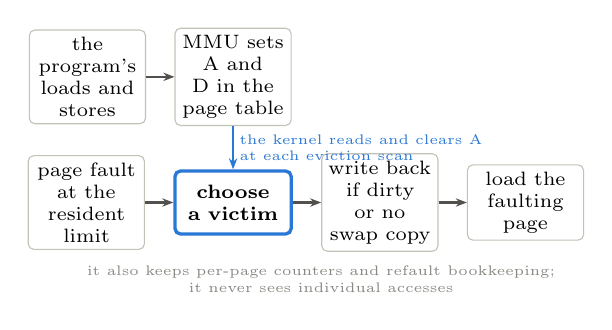
\begin{tikzpicture}[font=\scriptsize, node distance=0.36cm,
  box/.style={draw=cAxis, rounded corners=2pt, align=center, inner sep=2.5pt,
    minimum height=0.8cm, text width=1.3cm},
  flow/.style={-{Stealth[length=4pt]}, cInk, thick}]
\node[box] (fault) {page fault at the resident limit};
\node[box, right=of fault, draw=cLin, very thick] (choose) {\textbf{choose a victim}};
\node[box, right=of choose] (wb) {write back if dirty or no swap copy};
\node[box, right=of wb] (load) {load the faulting page};
\node[box, above=0.55cm of choose] (mmu) {MMU sets A and D in the page table};
\node[box, left=of mmu] (prog) {the program's loads and stores};
\draw[flow] (prog) -- (mmu);
\draw[flow] (fault) -- (choose); \draw[flow] (choose) -- (wb); \draw[flow] (wb) -- (load);
\draw[flow, cLin] (mmu) -- node[right, text=cLin, font=\tiny, align=left, inner sep=2pt]
  {the kernel reads and clears A\\at each eviction scan} (choose);
\node[below=0.06cm of wb.south west, anchor=north, text=cMuted, font=\tiny, align=center]
  {it also keeps per-page counters and refault bookkeeping;\\it never sees individual accesses};
\end{tikzpicture}
% Drawn from kernel/vmpage.c reclaim_frame() and sample_page(); kernel/vm.c sets PTE_A at fault-in.
\caption{The eviction path. The policy decides once per eviction, on the fault path,
and sees only the accessed and dirty bits a scan finds, never individual accesses.}
\label{fig:mechanism}
\end{figure}

\subsection{Heuristics Leave Large Headroom}
\label{sec:bg-headroom}

\obs{1}{\clock is as good as exact LRU, and both are far from optimal.}
On the six workloads used for training (\S\ref{sec:eval-setup}), \clock is within 2\%
of exact LRU on five, xv6's Aging is barely better than FIFO, and exact LFU, which beats
\clock by 6--13\% on btree, reaches about 3$\times$ \clock, where our runs stop, on graph,
sort and matmul. \belady needs 43--54\% fewer faults
than \clock on the B-tree, key-value and graph workloads, 53--59\% on LZW, 38\% on
matmul, and only 10--17\% on sort (Figure~\ref{fig:headroom}).
$\rightarrow$ \emph{Recency and frequency both carry signal, but every fixed combination
fails on some workload; a policy should learn the combination.}
% src: ML_REPORT 6.1 classical_test / classical_heldout (simulator, geo-mean 5/10/20%);
% report/results2/summary_classical.csv: lfu_exact btree 0.943 test / 0.871 held-out; graph test,
% matmul and sort held-out 3.000 (censored at 3x), sort test 2.919 (5 censored cells). Note LRU
% beats Clock on matmul (0.879), so "the only classical policy that beats Clock" was wrong.
% classical results unchanged by the week-15 refit (AUSTRA_HANDOFF.md, week-15 addendum).
% src: lzw Belady 0.466 (test) / 0.409 (held-out), week_16 tables/model_comparison.tex

\begin{figure}[t]
\centering
\begin{tikzpicture}
\begin{axis}[paperplot, width=\linewidth, height=1.42in, tick pos=left,
  xmin=0.25, xmax=1.56, ymin=-0.6, ymax=5.6, y dir=reverse,
  ytick={0,...,5}, yticklabels={btree,graph,kv,lzw,matmul,sort},
  xtick={0.4,0.6,0.8,1.0,1.2,1.4}, xmajorgrids,
  xlabel={faults relative to \clock}, xlabel style={yshift=3pt},
  legend style={at={(0.5,1.02)}, anchor=south, legend columns=-1,
    /tikz/every even column/.append style={column sep=6pt}}]
\addplot[cInk, thin, forget plot] coordinates {(1,-0.6) (1,5.6)};
\addplot[only marks, mark=*, mark size=1.5pt, cInk, fill opacity=0.75, draw opacity=0.75]
  table[x=ratio, y=row, col sep=comma] {\figdata/headroom_classical.csv};
\addlegendentry{FIFO, Aging, LFU, LRU, exact LFU}
\addplot[only marks, mark=triangle*, mark size=2pt, mark options={rotate=-90}, cInk,
  forget plot] table[x=ratio, y=row, col sep=comma] {\figdata/headroom_clipped.csv};
\addplot[only marks, mark=*, mark size=2.2pt, cLin,
  error bars/.cd, x dir=plus, x explicit, error mark=none,
  error bar style={cLin, line width=1.2pt}]
  table[x=ratio, y=row, x error=gap, col sep=comma] {\figdata/headroom_belady.csv};
\addlegendentry{\belady}
\addplot[only marks, mark=none, nodes near coords, point meta=explicit symbolic,
  every node near coord/.append style={anchor=east, font=\tiny, text=cLin, xshift=-2pt},
  forget plot]
  table[x=ratio, y=row, meta=label, col sep=comma] {\figdata/headroom_belady.csv};
\end{axis}
\end{tikzpicture}
% data: figures/data/headroom_*.csv from report/results2/summary_classical.csv (make_figdata.py)
\caption{Headroom (simulator, geometric mean over 5, 10 and 20\% memory; test streams,
matmul held-out). The blue rule is the gap between \belady and the best classical
policy. Exact LFU, whose runs stop at 3$\times$ \clock's faults, is drawn at the edge.}
\label{fig:headroom}
\end{figure}

\subsection{The Kernel's Coarse Signals Carry the Information}
\label{sec:bg-signals}

\obs{2}{What the kernel can sample nearly matches what an oracle trace records.}
We rank each feature against the true next-use distance \emph{within} each eviction
decision, because choosing among the candidates of one decision is all a policy does.
Measured that way, the kernel's sampled access count \feat{sfreq} is about as
informative as the exact count \feat{freq} that only a full trace gives (mean over the
six training workloads $-0.27$ vs.\ $-0.24$; btree $-0.53$ vs.\ $-0.59$, kv $-0.47$ vs.\
$-0.54$), and the refault distance that Linux's workingset code already measures is the
strongest of the three ($+0.32$) (Figure~\ref{fig:diagnostics}).
$\rightarrow$ \emph{Use kernel-observable features, and train and judge them on eviction
decisions, not on individual references} (\S\ref{sec:design-features},
\S\ref{sec:design-train}).
% src: report/results2/feature_diagnostics.csv (regenerated 2026-10-08, deterministic seeds),
% values from GAWWY_HANDOFF_PAPER.md reply M4 (Spearman, mean over six workloads).

\begin{figure}[t]
\centering
\begin{tikzpicture}
\begin{axis}[paperplot, diverging, width=0.72\linewidth, height=1.15in,
  scale only axis, enlargelimits=false, clip=false,
  xmin=-0.5, xmax=11.5, ymin=-0.5, ymax=6.5, y dir=reverse,
  xtick={0,...,11}, xticklabels={rec,freq,sd,wr,ref,aging,sfreq,idle,age,dirty,refaults,rdist},
  xticklabel style={font=\tiny\ttfamily, rotate=40, anchor=north east, inner sep=1pt},
  ytick={0,...,6}, yticklabels={btree,graph,kv,lzw,matmul,sort,\textbf{mean}},
  yticklabel style={font=\tiny}, tick style={draw=none}, axis line style={draw=none},
  point meta min=-0.7, point meta max=0.7,
  colorbar, colorbar style={width=4pt, ytick={-0.6,0,0.6}, font=\tiny,
    yticklabel style={font=\tiny}, axis line style={cAxis}}]
\addplot[matrix plot*, mesh/cols=12, point meta=explicit]
  table[x=col, y=row, meta=rho, col sep=comma] {\figdata/diagnostics.csv};
\addplot[only marks, mark=none, nodes near coords, point meta=explicit symbolic,
  every node near coord/.append style={anchor=center, font=\tiny, yshift=0pt}]
  table[x=col, y=row, meta=label, col sep=comma] {\figdata/diagnostics.csv};
\draw[white, line width=1.6pt] (axis cs:3.5,-0.5) -- (axis cs:3.5,6.5);
\draw[white, line width=1.6pt] (axis cs:9.5,-0.5) -- (axis cs:9.5,6.5);
\draw[white, line width=1.6pt] (axis cs:-0.5,5.5) -- (axis cs:11.5,5.5);
\node[font=\tiny, text=cMuted, anchor=south] at (axis cs:1.5,-0.55) {oracle (\tierF)};
\node[font=\tiny, text=cMuted, anchor=south] at (axis cs:6.5,-0.55) {kernel scans (\tierK)};
\node[font=\tiny, text=cMuted, anchor=south] at (axis cs:10.5,-0.55) {refaults (\tierKp)};
\end{axis}
\end{tikzpicture}
% data: figures/data/diagnostics.csv from report/results2/feature_diagnostics.csv (make_figdata.py)
\caption{Rank correlation of each feature with the next-use distance within each
eviction decision (Spearman; red: a larger value means a later next use). The kernel's
\feat{sfreq} is as informative as the trace-only \feat{freq}; \feat{rdist} beats both.}
\label{fig:diagnostics}
\end{figure}

\subsection{A Naively Trained Policy Fails}
\label{sec:bg-naive}

\obs{3}{Trained on uniformly sampled candidates, a learned policy evicts the page the
program is streaming through.}
With \belady's choice plus 31 uniformly sampled candidates per recorded eviction, two
thirds of the linear models trained on graph (203 of 300 feature sets) make at least
3$\times$ \clock's faults on a PageRank stream at 10\% memory; in the first version of this study, three
rounds of DAgger~\citep{ross2011dagger} did not help. A failing model evicts what it has
just loaded: 86--87\% of its victims had been loaded at the immediately preceding fault
and were needed again a median of 15--16 references later, while \belady's choice at the
same decisions had last been used a median of 234--270 references earlier. Out of 167
resident pages, the one or two just touched are almost never sampled, so the model never
learned to keep them.
$\rightarrow$ \emph{The training distribution must contain just-used pages, and new pages
need protection} (\S\ref{sec:design-train}).
% src: report/results2/r3_first_version.md (R3, rerun 2026-10-13 with the current seeds:
% first-version data, no probation; graph-pr2000x2-s2 at 10%, 167 frames; median model and
% all-features model: 85.7% / 87.3% loaded at the previous fault, next use 15 / 16, Belady's
% choice last used 270 / 234 earlier; best of 300: 0.762x Clock, 0.9%). DAgger three rounds:
% ML_REPORT 7.3, first version, not rerun. Text only, no figure (space).

\subsection{Research Questions}
\label{sec:bg-rq}

Whether a learned policy is implementable in a kernel breaks into four questions,
answered in \S\ref{sec:eval}:
\begin{description}[topsep=2pt, itemsep=1pt, parsep=0pt]
\item[RQ1 Information.] Do kernel-observable signals suffice, or does a learned policy
  need information only a full trace has? (\S\ref{sec:eval-info})
\item[RQ2 Effect in the kernel.] Inside a real kernel, does the policy beat \clock and
  the strongest classical policies a kernel can run, across memory sizes?
  (\S\ref{sec:eval-kernel})
\item[RQ3 Cost.] Can it be computed without floating point, what does a decision cost
  on the eviction path, and when does a saved fault pay for it? (\S\ref{sec:eval-cost})
\item[RQ4 Robustness.] What happens on workloads it never saw, and where does it fail?
  (\S\ref{sec:eval-robust}, \S\ref{sec:eval-loss})
\end{description}
%==============================================================================
% ----- 3 DESIGN -----
%==============================================================================
% =============================================================================
\section{Learning From What the Kernel Already Sees}
\label{sec:design}
% Budget: 3.0 pages. Draft SECOND (Step 5.2). One subsection per challenge, each
% "Observation. -> Solution." Misprediction handling is its own subsection.
% Self-check: a reader can follow ONE eviction step by step; the worst case under a
% bad model is stated; every named component appears in the evaluation.
% =============================================================================

\subsection{Overview and Formulation}
\label{sec:design-overview}

\finding{Offline.} Each training stream, a complete reference string
(\S\ref{sec:impl}), is replayed under LRU at 5, 10 and 20\% of its distinct pages. At a
sample of evictions we record the resident candidates with their features and labels
(\S\ref{sec:design-train}), fit a linear scorer, choose the feature subset and the
probation length on validation streams only, and export the weights as integers
(Figure~\ref{fig:overview}).
\finding{Online.} At each eviction the kernel scans the eligible resident pages as Aging
already does, updates their counters, scores each with an integer dot product, skips
pages in probation, and evicts the highest score, the oldest load on a tie
(Algorithm~\ref{alg:choose}).

\finding{Formulation.} The policy imitates \belady. For each candidate it predicts
$\log(1+d)$, where $d$ is the number of references until the page's next use, capped at
$2^{20}$, and it evicts the candidate with the largest prediction; the fit is
closed-form ridge regression. Supervised imitation suits the problem because complete
reference strings give exact labels offline and \belady is optimal for faults;
reinforcement learning would have to explore inside a running kernel. Decisions
compound, so every policy is judged by replaying complete streams, never by
per-reference accuracy. The global model is trained on six workloads (B-tree, graph,
key-value, LZW, matmul, sort) and used unchanged on all others. It is linear because
five heavier models trained the same way do no better at 20--150$\times$ the cost
(\S\ref{sec:eval-ablate}).
% src: tools/ml2/build_datasets.py (LRU replay, MAX_CAND 32, N_RECENT 4, label log1p capped);
% tools/ml2/pagesim.c LABEL_CAP (1 << 20); tools/ml2/models.py ("closed-form weighted ridge
% regression"); kernel/vmpage.c choose_ml(); selection on validation: ML_REPORT 5.2, 7.2.

\begin{figure*}[t]
\centering
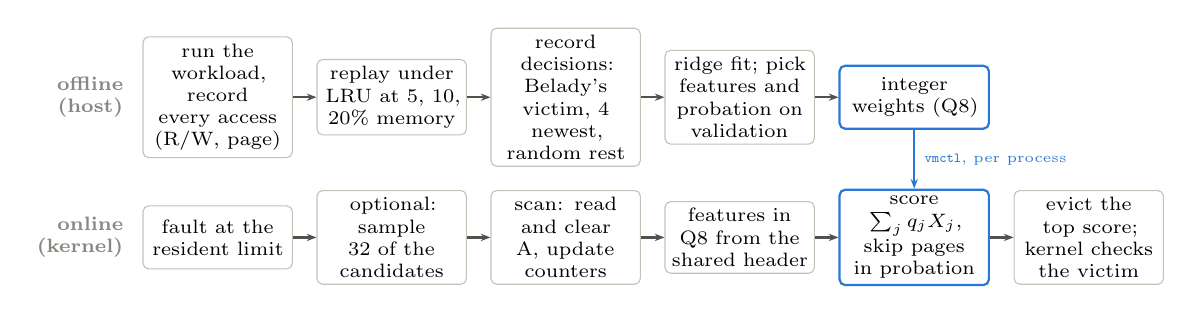
\begin{tikzpicture}[font=\scriptsize, node distance=0.3cm,
  box/.style={draw=cAxis, rounded corners=2pt, align=center, inner sep=2.5pt,
    minimum height=0.8cm, text width=1.72cm},
  flow/.style={-{Stealth[length=3.5pt]}, cInk, thick},
  lane/.style={font=\scriptsize\bfseries, text=cMuted, anchor=east, align=right}]
% offline row
\node[box] (o1) {run the workload, record every access (R/W, page)};
\node[box, right=of o1] (o2) {replay under LRU at 5, 10, 20\% memory};
\node[box, right=of o2] (o3) {record decisions: \belady's victim, 4 newest, random rest};
\node[box, right=of o3] (o4) {ridge fit; pick features and probation on validation};
\node[box, right=of o4, draw=cLin, thick] (o5) {integer weights (Q8)};
% online row
\node[box, below=0.6cm of o1] (k1) {fault at the resident limit};
\node[box, right=of k1] (k2) {optional: sample 32 of the candidates};
\node[box, right=of k2] (k3) {scan: read and clear A, update counters};
\node[box, right=of k3] (k4) {features in Q8 from the shared header};
\node[box, right=of k4, draw=cLin, thick] (k5) {score $\sum_j q_j X_j$, skip pages in probation};
\node[box, right=of k5] (k6) {evict the top score; kernel checks the victim};
\foreach \a/\b in {o1/o2,o2/o3,o3/o4,o4/o5,k1/k2,k2/k3,k3/k4,k4/k5,k5/k6}
  \draw[flow] (\a) -- (\b);
\draw[flow, cLin] (o5) -- node[right, font=\tiny, text=cLin] {\texttt{vmctl}, per process} (k5);
\node[lane, left=0.12cm of o1] {offline\\(host)};
\node[lane, left=0.12cm of k1] {online\\(kernel)};
\end{tikzpicture}
% Drawn from tools/ml2/build_datasets.py (LRU replay, MAX_CAND 32, N_RECENT 4), models.py (ridge),
% export_kernel.py (integer weights), kernel/vmpage.c choose_ml()/ml_sample(), kernel/mlfeat.h.
\caption{Overview. Training is offline and uses the future; the kernel side is a scan it
already performs plus a few integer multiply-adds per page.}
\label{fig:overview}
\end{figure*}

% -----------------------------------------------------------------------------
\subsection{Features the Kernel Already Keeps}
\label{sec:design-features}
% Challenge C1 -> technique T1 -> ablation A1 (tier comparison, Table tab:tiers)

\finding{Observation.} A kernel never sees individual accesses
(\S\ref{sec:bg-mechanism}), so a model trained on per-access recency or frequency cannot
be deployed as trained.

\finding{Solution.} The policy uses only features a kernel can compute when it scans the
resident pages at an eviction (tier \tierK), plus refault bookkeeping that Linux already
keeps in its workingset shadow entries (tier \tierKp) (Table~\ref{tab:features}). Time is
counted in scans, one per eviction. Counts enter as $\log(1+x)$ and are standardised.
Oracle features (tier \tierF: exact recency, frequency, stack distance, write ratio)
serve only as an ablation that bounds what extra information is worth.

\begin{table}[t]
\caption{Kernel-observable features. All are small per-page integers; the last column
names the Linux state that already holds an equivalent.}
\label{tab:features}
\vskip 0.1in
\begin{center}
\begin{footnotesize}
\setlength{\tabcolsep}{3pt}
\begin{tabular}{@{}l>{\raggedright\arraybackslash}p{1.2in}>{\raggedright\arraybackslash}p{1.15in}@{}}
\toprule
Feature & Definition & Linux analogue \\
\midrule
\multicolumn{3}{@{}l}{\textit{\tierK: from accessed/dirty-bit scans}}\\
\feat{ref}      & A bit at this scan                     & young bit, PG\_referenced \\
\feat{aging}    & 8-bit aging counter                    & -- \\
\feat{sfreq}    & scans that found it accessed           & DAMON access count; MGLRU tiers \\
\feat{idle}     & scans since last found accessed        & MGLRU generation age; DAMON age \\
\feat{age}      & scans since it was loaded              & -- \\
\feat{dirty}    & D bit                                  & PG\_dirty \\
\midrule
\multicolumn{3}{@{}l}{\textit{\tierKp: refault bookkeeping}}\\
\feat{refaults} & times evicted and faulted back         & workingset shadow entry \\
\feat{rdist}    & evictions between its eviction and refault & workingset refault distance \\
\bottomrule
\end{tabular}
\end{footnotesize}
\end{center}
\vskip -0.1in
\end{table}
% src: ML_REPORT section 4 and 9. Linux versions (checked 2026-10-13, kernelnewbies): MGLRU
% merged in 6.1 (Dec 2022), DAMON in 5.15 (Oct 2021); ML_REPORT's "5.18+" for MGLRU was wrong.

% -----------------------------------------------------------------------------
\subsection{Training on Decisions, Not References}
\label{sec:design-train}
% Challenge C3 -> technique T3 -> ablations A3 (v1 vs v2; probation sweep; DAgger)

\finding{Observation.} A policy acts at an eviction, over the pages resident at that
moment, and a naive sample of those pages almost never contains the page just used
(\S\ref{sec:bg-naive}).

\finding{Solution.} The policy is trained on recorded eviction decisions. Every training and
validation stream is replayed under LRU at 5, 10 and 20\% of its distinct pages; at a
sample of evictions we record up to 32 resident candidates with their features and
labels: always \belady's victim, always the four most recently accessed candidates
(recency-stratified recording), and the rest uniformly. This raises the share of
just-accessed rows from 0.6\% to 3.1\%. Second, a \emph{probation} rule: a page loaded
fewer than $p$ scans ago is not evicted while an older candidate exists, which is
\clock's second chance applied to a learned score. $p\in\{0,1,2,4\}$ is chosen per
scope on validation. Over the six training workloads this gives 5.22M training rows
from 377K decisions, and 0.91M validation rows from 43K decisions.
% src: GAWWY_HANDOFF_PAPER.md reply M5 (dataset_summary.csv): train 5,216,668 rows / 376,706
% decisions; validation 912,604 / 42,653 (total 6,129,272 / 419,359). Method: ML_REPORT 5.2, 7.2.

% -----------------------------------------------------------------------------
\subsection{Integer-Only Scoring}
\label{sec:design-int}
% Challenge C2 -> technique T2 -> ablations A2 (float vs 4/8/12-bit; linear vs MLP)

\finding{Observation.} xv6 saves no floating-point registers on a context switch, and
Linux normally prohibits kernel code from using floating point outside an explicit
critical section~\citep{linux_fpu}.
% src: kernel/swtch.S (ra, sp, s0-s11 only); docs.kernel.org/core-api/floating-point.html
% ("Kernel code is normally prohibited from using floating-point (FP) registers or
% instructions"; kernel_fpu_begin/end), checked 2026-10-13.

\finding{Solution.} The score of a candidate page is
\begin{equation}
s(\text{page}) = \sum_{j\in S} q_j\, X_j(\text{page}), \qquad
q_j = \operatorname{round}\!\left(\frac{w_j}{\sigma_j}\, 2^{b}\right),
\label{eq:score}
\end{equation}
where $X_j$ is feature $j$ in Q8 fixed point, $S$ is the selected subset (1--5
features), and the standardisation is folded into the weight. Means and the bias are the
same for every candidate and drop out of the arg-max. $\log(1+x)$ comes from a 256-entry
table plus a most-significant-bit search and a 1,024-entry mantissa table, within 1.04
Q8 units of exact. The same header computes features in the kernel and in the
simulator, so a model scores a page identically in both. The kernel's default weights
are the global model over five features (\feat{idle}, \feat{age}, \feat{dirty},
\feat{refaults}, \feat{rdist}; probation 4 scans).

\finding{Heavier models, in whole numbers too.} To test whether capacity pays, five
heavier models (a CNN over the aging bits, a deeper MLP, set-attention, boosted trees and
ranking trees) are converted to whole-number arithmetic with a shared evaluator that the
kernel and the simulator both compile, and selected per process like the linear weights.
% src: ML_REPORT 8, 8b; kernel/mlweights.h (current default); kernel/mlnet.h; AUSTRA_HANDOFF week-15 addendum

% -----------------------------------------------------------------------------
\subsection{When the Model Is Wrong}
\label{sec:design-wrong}
% Challenge C4 -> technique T4 -> ablation A4 (deliberately wrong models). NON-NEGOTIABLE.
% Every accepted ML-for-OS paper has a design element here, not a sentence.

The worst case is a policy that makes more faults than \clock; it is never wrong data.
Three layers keep it there.
\begin{enumerate}
\item \textbf{Correctness never depends on the model.} The score only orders eligible
  candidates (the faulting process's own evictable frames). The kernel checks every
  returned victim against that set and falls back to \clock if it is not in it. A bad
  model costs performance, not data (\S\ref{sec:impl}); the fallback never fired in any
  correctness run (all nine policies and the five heavier models, with and without
  prefetch).
  % src: GAWWY_HANDOFF_PAPER.md reply M5; R4 (LeCaR passes data invariance, 0 fallbacks).
  % The evaluation transcripts do not record the counter, so there is no sum over the
  % 3,257 runs; say "correctness runs", not "all runs".
\item \textbf{Probation} keeps the newest pages out of the choice, removing the failure
  of \S\ref{sec:bg-naive}.
\item \textbf{Validation-only selection.} Many feature sets are catastrophic: at 10\%
  memory, 113 of the 300 sets reach $3\times$ \clock or more on graph and 52 on kv.
  Feature set and probation are chosen jointly on validation, never on test or held-out
  streams.
  % src: tables.md "catastrophic" (v2, test split), regenerated; GAWWY_HANDOFF_PAPER.md reply M4
\end{enumerate}
Nothing switches the policy off at run time, so the learned score can still be worse
than \clock on a workload; \S\ref{sec:eval-loss} lists where, and those losses are what a
deployment would see.
% The simulator guard prototype was DROPPED by the collaborator (AUSTRA_HANDOFF.md START HERE
% 2b): not in the kernel, not to be presented as future work. Do not reintroduce it.

% -----------------------------------------------------------------------------
\subsection{Bounding the Decision Cost}
\label{sec:design-cost}
% Challenge C5 -> technique T5 -> ablation A5 (sample size k vs faults and instructions).

\finding{Observation.} Scoring every eligible page costs about 340 instructions per
candidate, so the decision grows in a straight line with the resident set
(\S\ref{sec:eval-cost}).

\finding{Solution.} Score only $k$ randomly sampled candidates, drawn with a partial
Fisher--Yates shuffle over the candidate array (no extra memory). With $k=32$ the
decision costs 11,300--11,900 instructions whatever the memory size, and at 10\% memory
it makes no measurably more faults; $k=16$ costs 5,660--5,970 for 1.3\% more on average
(\S\ref{sec:eval-ablate}). The weights are unchanged; $k$ is a per-process setting.
% src: cost_grid.csv (global@32: 11,293 / 11,813 / 11,907 at 64 / 256 / 512 frames; @16:
% 5,656 / 5,914 / 5,974); ci_main.tex R1 rows (74 streams, 10%, global weights: 32 sampled vs
% full 0.998 [0.97, 1.02]; 16 sampled 1.013 [0.98, 1.04], interval includes 1)

% -----------------------------------------------------------------------------
\begin{algorithm}[t]
\caption{Victim selection by the learned score (\texttt{choose\_ml}), one eviction}
\label{alg:choose}
\begin{algorithmic}
\STATE {\bfseries Input:} eligible resident pages $C$, weights $q$, subset $S$, probation $p$, scan counter $t$
\STATE {\bfseries if} sample size $k$ is set {\bfseries then} $C \leftarrow k$ random pages of $C$ \hfill (partial Fisher--Yates)
\STATE $old \leftarrow$ false; \ $best \leftarrow \bot$
\FOR{each page $c \in C$}
  \STATE read and clear $A(c)$; update \feat{aging}, \feat{sfreq}, last-seen scan
  \STATE {\bfseries if} $t - \mathrm{load}(c) \ge p$ {\bfseries then} $old \leftarrow$ true
\ENDFOR
\STATE flush the TLB once if any A bit was cleared
\FOR{each page $c \in C$}
  \IF{$old$ {\bfseries and} $t - \mathrm{load}(c) < p$}
    \STATE skip $c$ \hfill (probation)
  \ENDIF
  \STATE $s_c \leftarrow \sum_{j\in S} q_j X_j(c)$ \hfill (integers, Q8)
  \STATE keep $c$ if $s_c > s_{best}$, or equal and loaded earlier
\ENDFOR
\STATE {\bfseries return} $best$ \hfill (kernel validates it; \clock if invalid)
\end{algorithmic}
\end{algorithm}
% src: kernel/vmpage.c choose_ml() (39 lines) and choose_policy_victim(); kernel/mlfeat.h (63 lines)
%==============================================================================
% ----- 4 IMPLEMENTATION -----
%==============================================================================
% =============================================================================
\section{Implementation}
\label{sec:impl}
% Budget: 0.5-0.75 page. Draft THIRD (Step 5.3). Self-check: a reviewer can estimate
% the overhead from this section alone; the simulator/real-kernel boundary is stated.
% DOUBLE-BLIND: no names, lab URLs, or repository paths that identify the authors.
% =============================================================================

\finding{A paging layer for xv6.} Stock \xv~\citep{xv6} allocates every page eagerly and
never evicts; it has no page-fault path for memory, no backing store and no
replacement policy. We added demand paging, a raw swap area outside the file system
(8,192 slots, 32\,MB), a frame table with per-process resident limits, FIFO, \clock,
Aging and a decayed LFU, synchronous and asynchronous prefetch, an event tracer, and a
control call (\texttt{vmctl}) that sets a process's limit, policy and weights: about
4,300 kernel lines over upstream xv6, all policies included. On the final build the same
workload produces byte-identical output under all nine policies and the five heavier
models, with and without prefetch. Why xv6, and what differs from Linux, is discussed in
\S\ref{sec:discussion}.
% src: git diff --stat 7d01506..HEAD -- kernel (4,317 insertions, 37 files; rechecked 2026-10-14,
% after LeCaR, R4); data invariance: GAWWY_HANDOFF_PAPER.md reply M5 and R4 (checksum AB0C8578
% everywhere, LeCaR included). The full
% 74-step regression matrix was NOT rerun on the final build (handoff "State of everything"):
% cite only data invariance.

\finding{The learned policy in the kernel.} \texttt{choose\_ml} (60 lines, with a 14-line
sampler) scans the candidates as Aging already does and scores them with
Equation~\ref{eq:score}; a 63-line header computes the Q8 features, and a 203-line
evaluator runs the heavier models in whole numbers. Both headers are compiled into the
kernel and the simulator. The learned policy's bookkeeping adds 40 bytes to each
resident page's record (120 to 160 bytes: load scan, last-seen scan, sampled count,
refault count, refault distance) and 12 bytes to each swap slot (the eviction time and
refault count, the information Linux keeps in a workingset shadow entry). The linear
weights are an 80-byte record per process, set through \texttt{vmctl} with the model and
sample size, and inherited across \texttt{fork} and \texttt{exec}. The ten built-in
heavier models take 100,716 bytes of read-only kernel data; the accessed-bit forms of
ARC, LHD and S3-FIFO share about 0.95\,MB of machine-wide state.
% src: kernel/vmpage.c (choose_ml, ml_sample), kernel/mlfeat.h, kernel/mlnet.h;
% sizes from GAWWY_HANDOFF_PAPER.md reply M5

\finding{Classical policies in accessed-bit form.} ARC, LHD and S3-FIFO react to
every hit, which a kernel never sees. Each was adapted the same way: accessed bits are
read and cleared at every eviction, and a page found accessed counts as one hit since the
last look (the touch that loaded it is ignored); everything else follows the published
algorithm (ARC's four lists, ghost lists and adaptive target; S3-FIFO's small, main and
ghost queues; LHD's per-class hit and eviction histograms, with time in evictions).
LeCaR~\citep{vietri2018lecar} is adapted the same way, with ghost lists as in ARC and
whole-number weights (its experts: \S\ref{sec:eval-info}). The four are 73, 34, 44 and 56
lines in the kernel. Their simulator versions match independent reference
implementations, faults and evictions alike (Appendix~\ref{app:sim}).
% src: week_16 report section "The three classical policies in the kernel"; kernel/vmpage.c
% choose_arck/s3fifo/lhd; choose_lecar (lines 785-840; weights in 2^30 units, regret factor from a
% 64-entry table; GAWWY_HANDOFF_PAPER.md R4)

\finding{Complete reference strings and a validated simulator.} Each workload routes
every access to its data through one accessor that records \texttt{R} or \texttt{W} and
the page number, so a stream is a complete reference string, which \belady labels
require; every string matches an independent model of its program. Feature selection
needs tens of thousands of full replays, so it runs in a C simulator, checked against
independent implementations and against the kernel's own logic and features, and started,
like the kernel's benchmarks, from filled memory (Appendices~\ref{app:data}
and~\ref{app:sim}).
% src: ML_REPORT 2.2-2.3, 5.1; week-16 report; details in Appendix A/B

\finding{Measuring cost and running at scale.} Decision cost is counted in instructions
with QEMU in instruction-counting mode, which repeats to within 0.3\%; the timer-tick
counters of ordinary runs are too noisy for cost. The 3,257 kernel runs were split
between one desktop and cloud notebooks; 180 runs repeated on both gave identical faults,
evictions and writes. Training is cheap: the linear score is a closed-form fit, and the
heavier models train in 2--67\,s (trees on a CPU, networks on one consumer GPU).
% src: AUSTRA_HANDOFF START HERE sections 2, 3, 6 (QEMU_ICOUNT; select_ticks not usable for cost);
% training times: GAWWY_HANDOFF_PAPER.md reply M5 (global scope; MLP 48 s, CNN 48 s, set-attention
% 67 s on an RTX 3060 Ti; boosted trees 1.8 s, ranking trees 2.7 s, CPU)

\finding{Availability.} The kernel, workloads, traces, simulator and training pipeline
will be released as open source and submitted for artifact evaluation
(Appendix~\ref{app:repro}); streams derived
from the Twitter traces will carry their CC~BY~4.0 licence and attribution.
\todo{anonymized code and data link for review (e.g.\ an anonymous mirror); the repository
history and names must not identify the authors}
% Twitter licence verified 2026-10-12 (GAWWY_HANDOFF_PAPER.md "Twitter licence"): CC BY 4.0;
% release only derived streams, with attribution and a change note; do not redistribute the
% original archive.
%==============================================================================
% ----- 5 EVALUATION -----
%==============================================================================
% =============================================================================
\section{Evaluation}
\label{sec:eval}
% Budget: 3.0 pages. Draft FOURTH (Step 5.4). Questions first; each figure answers one
% question and its caption states the answer. Oracle (Belady) where it exists. Intervals
% on main results. Losses stated.
% NUMBERS: the kernel tables are \input from report/week_16_update/tables (generated by
% tools/ml2/report_w15.py + report_w16.py from report/results2); never retype them.
% Numbers quoted in the text carry a "% src:" comment. Status FINAL unless marked.
% =============================================================================

We answer the four questions of \S\ref{sec:bg-rq}: RQ1 information
(\S\ref{sec:eval-info}), RQ2 effect inside the kernel (\S\ref{sec:eval-kernel}), RQ3
cost (\S\ref{sec:eval-cost}) and RQ4 robustness (\S\ref{sec:eval-robust}), then the
ablations (\S\ref{sec:eval-ablate}) and where the learned policy does not help
(\S\ref{sec:eval-loss}).

% -----------------------------------------------------------------------------
\subsection{Setup}
\label{sec:eval-setup}

\finding{Platform.} \xv on QEMU 8.2.2 (\texttt{virt} machine, one hart, 128\,MB), built
with GCC 13.3, on a 6-core desktop CPU under Ubuntu 24.04. A kernel run repeats exactly:
the same program, stream, memory size and policy give the same faults every time, so the
uncertainty we report comes from which streams were run, not from run-to-run noise.

\finding{Workloads.} Fourteen (Table~\ref{tab:workloads}). The learned models are trained
on six of them (B-tree, graph, key-value, LZW, matmul, sort) and run unchanged on the
other eight, which include an eleven-pattern synthetic suite with known answers,
application-shaped programs, and our key-value store replaying six Twitter cache
clusters~\citep{yang2020twitter} (4, 17, 18, 24, 35, 52, from the archive of
\citet{zussman2025cacheext}), each sampled by key hash to about 1,000 keys and cut to
4,751--40,000 requests; only key ids and write flags are kept.

\finding{Memory and runs.} The resident limit is 5, 10 or 20\% of each program's pages,
with the same 74 streams at every size; the pattern and application programs run their
first 50,000 accesses. 3,257 kernel runs in total.
% src: week_16 report section "What was run"; AUSTRA_HANDOFF START HERE sections 2, 6 (round 5
% added 23 streams at 5% and 20%); rounds 6-7 (R1, R2: 440 runs; R4 LeCaR: 74 runs) bring
% kernel_eval_all.csv to 3,257 rows; Twitter: GAWWY_HANDOFF_PAPER.md "Twitter licence" (CC BY 4.0;
% the text must say the data were changed), tools/gen_tw_keys.py, user/twk{4,17,18,24,35,52}.bin

\finding{Policies.} In the kernel: FIFO, \clock, Aging, LFU; ARC~\citep{megiddo2003arc},
LHD~\citep{beckmann2018lhd} and S3-FIFO~\citep{yang2023s3fifo} in accessed-bit form
(\S\ref{sec:impl}); the learned linear score with one global set of weights (per-workload
weights where stated), also with 32 and 16 sampled candidates; five heavier models trained
on the same six workloads; and LeCaR~\citep{vietri2018lecar}, the closest learned-cache
baseline, in accessed-bit form. The heavier models ran on all 74 streams at 10\% memory
and on ten at 5\% and 20\%, LeCaR at 10\% only. \belady, and LeCaR as published, appear
only in simulation.

\finding{Metrics.} Faults are zero-fill plus swap faults, relative to \clock on the same
stream and memory. We average with a geometric mean over the streams of each workload,
then over the 14 workloads with equal weight, so a workload with 17 streams counts once.
95\% intervals resample the workloads, then the streams inside them. Decision cost is in
instructions, counted exactly (\S\ref{sec:impl}), with 68 candidates per eviction. Page
writes (write-backs to swap) are averaged the same way as faults.
% src: week_16 report Summary and section "What was run"; AUSTRA_HANDOFF START HERE sections 0, 6;
% platform: GAWWY_HANDOFF_PAPER.md reply M5 (QEMU 8.2.2, -machine virt -smp 1 -m 128M; Ryzen 5 5600;
% Ubuntu 24.04 on WSL2; riscv64-linux-gnu-gcc 13.3.0)

\begin{table}[t]
\caption{Workloads. The learned models are trained on the six marked ``train'' and run
unchanged on the other eight.}
\label{tab:workloads}
\vskip 0.1in
\begin{center}
\begin{footnotesize}
\setlength{\tabcolsep}{3pt}
\begin{tabular}{@{}l>{\raggedright\arraybackslash}p{1.95in}l@{}}
\toprule
Workload & What it is & Training \\
\midrule
btree  & B+-tree, 4\,KB nodes (SQLite-pager-like)                & train \\
graph  & BFS and PageRank, scale-free graph                       & train \\
kv     & Zipfian hash table, YCSB mixes (Redis-like)              & train \\
lzw    & LZW compression (\texttt{compress(1)})                   & train \\
matmul & naive vs.\ blocked matrix multiply                       & train \\
sort   & bottom-up merge sort                                     & train \\
\midrule
kv-T   & kv replaying Twitter cache traces                        & -- \\
heap   & \texttt{malloc}/\texttt{free} churn                      & -- \\
join   & hash join, build and probe                               & -- \\
spmv   & sparse matrix--vector product (CSR)                      & -- \\
chase  & serial pointer chasing                                   & -- \\
bloom  & Bloom-filter probes                                      & -- \\
pat    & 11 synthetic patterns (loop, Zipf, phase, \ldots)        & -- \\
app    & four application-shaped programs                         & -- \\
\bottomrule
\end{tabular}
\end{footnotesize}
\end{center}
\vskip -0.1in
\end{table}
% src: week_16 report "Workloads (14)"; week-15 report "New workloads"; GAWWY_HANDOFF_NEW_BENCHMARKS.md
% Credits (D2): the programs lzw, chase, join, bloom, spmv and heap are credited to their
% author in the camera-ready only (the blind version cannot name authors).

% -----------------------------------------------------------------------------
\subsection{RQ1: Does the Kernel See Enough?}
\label{sec:eval-info}
% Simulator results (the kernel cannot run oracle-input models). Filled-memory start.

\finding{With kernel signals only, more capacity does not help.} Boosted trees over the
same kernel-visible signals tie the linear score where both work (btree test 0.834 vs.\
0.835) and lose where data are scarce (LZW held-out 1.068 vs.\ 0.813; matmul held-out
0.803 vs.\ 0.671). Over all six workloads they are worse on test streams (0.897 vs.\
0.877) and level on held-out ones (0.894 vs.\ 0.896) (Appendix, Table~\ref{tab:info}).

\finding{Oracle inputs help only on familiar workloads.} Given information a kernel never
has (exact recency, frequency, reuse history), the best trees and networks are 2--5\%
better than the best linear score on the workloads they were trained on. On real Redis
and SQLite traces, recorded on Linux, every richer model is 22--41\% worse than the
linear one, and a linear score with oracle inputs reaches $3\times$ \clock on Redis.
What the kernel cannot see is not what limits a learned policy here; what it can see
transfers better.
% src: week-15 report "What the wider comparison says" and "Transfer to unseen workloads";
% week_16 tables/model_comparison.tex and tables/transfer.tex (redis-real linear F+K 3.000)

\finding{A learned-cache baseline needs what the kernel lacks.}
LeCaR~\citep{vietri2018lecar}, run as published with exact LRU and LFU as its two
experts, which needs every access, is 0.958 of \clock on the held-out streams of the six
workloads, against 0.896 for the linear score. In accessed-bit form, with \clock and the
kernel's decayed frequency count as experts, it is 1.116 in simulation (Appendix,
Table~\ref{tab:lecar}) and 1.113 in the kernel over 74 streams at 10\% memory (interval
1.04--1.23), worst on graph (1.60) and SpMV (1.47); its frequency expert alone, the
kernel's LFU, is 1.13. The linear score incurs 0.822 of LeCaR's faults (0.73--0.91).
% src: report/week_16_update/tables/lecar.tex ("global, held-out" row); GAWWY_HANDOFF_PAPER.md
% reply S3 (original parameters; checked against an independent reference on 95 traces).
% Kernel: R4 (kernel_eval_lecar.csv merged; ci_main.tex LeCaR rows; per workload graph 1.60,
% SpMV 1.47); LFU 1.13 = kmain_A_01 mean.

\finding{\feat{idle} carries the policy.} Adding \feat{idle} (scans since the page was
last found accessed) to a feature subset that lacks it cuts faults by a median of 71\% on
graph, 30\% on btree and 19\% on kv, though only 1\% on LZW (Appendix,
Figure~\ref{fig:marginal}). This is the signal MGLRU generations and DAMON ages already
track.
% src: report/results2/summary_marginal.csv (current), via GAWWY_HANDOFF_PAPER.md reply M4
% Table tab:info moved to the appendix (2026-10-14) to keep the body at 10 pages after R1-R6;
% the RQ1 text above quotes its key numbers.


% -----------------------------------------------------------------------------
\subsection{RQ2: Does It Work Inside the Kernel?}
\label{sec:eval-kernel}

\begin{table*}[t]
\caption{\textbf{Every policy on every workload, in the xv6 kernel, at 10\% memory} (74
streams). Faults relative to \clock: one column per workload (geometric mean over its
streams), last column the mean over the 14 workloads. ARC, LHD and S3-FIFO in
accessed-bit form. The 5\% and 20\% tables are in Appendix~\ref{app:results}.}
\label{tab:kernel}
\vskip 0.1in
\begin{center}
\resizebox{\textwidth}{!}{\input{\wsixteen/kmain_A_01}}
\end{center}
\vskip -0.1in
\end{table*}

\begin{table}[t]
\caption{The comparisons that matter, with 95\% intervals (resampling workloads, then
streams). Bold: the whole interval is below 1. Every 10\% cell covers 74 streams; at 5\%
and 20\% the heavier models ran on ten. All comparisons: Table~\ref{tab:ci-full}.}
\label{tab:ci}
\vskip 0.1in
\begin{center}
\resizebox{\linewidth}{!}{\input{\figdata/ci_body.tex}}
\end{center}
\vskip -0.1in
\end{table}
% data: figures/data/ci_body.tex = the rows of week_16 tables/ci_main.tex the body cites, written by
% make_figdata.py from kernel_ci_classic.csv in the same format (the full table is tab:ci-full).

\finding{The linear score beats \clock at 10\% memory} (0.914, interval 0.85--0.98;
Table~\ref{tab:ci}). At 5\% (0.976) and 20\% (0.882) it is better on average, but the
intervals include 1 (at 20\% only just): a few workloads decide the average.

\finding{It is level with ARC, not better.} ARC, in accessed-bit form, beats \clock at 5\%
and 10\% (0.947 and 0.943, intervals below 1) and is level at 20\% (0.984). The linear
score against ARC is 1.031, 0.970 and 0.896 at 5, 10 and 20\% memory; no interval
excludes 1, and the gap moves in the learned score's favour as memory grows. LHD is the
most uneven (0.63 on graph at 10\%, level elsewhere); S3-FIFO in accessed-bit form is not
better than \clock at any size; FIFO, Aging and LFU are worse than \clock at every size,
by 4--35\% on average.
% src: ci_main.tex / kernel_ci_classic.csv after round 5 (linear vs Clock at 20%: [0.766, 1.001]);
% kmain_A_* mean column (FIFO/Aging/LFU 1.04-1.35)

\finding{Where it wins.} The learned score does best where recency is a poor guide:
btree and kv (0.82--0.96 at every size), the heap programs (0.73 at 10\%, 0.56 at 20\%),
pointer chasing, and the hash join at 20\% (0.55) (Table~\ref{tab:kernel}).

\finding{Page writes do not fall on average.} The learned score is trained to save faults,
not writes: its label is \belady's next-use distance. Against \clock its page writes are
1.215, 1.120 and 0.984 at 5, 10 and 20\% memory, and every interval includes 1 ([0.85,
2.05], [0.84, 1.74], [0.72, 1.51]). At 10\% it writes less on btree (0.95), kv (0.78),
heap (0.72) and pointer chasing (0.73), but 4.75$\times$ \clock on matmul and 4.22$\times$
on SpMV, which pull the mean up. ARC writes less than \clock at 5\% and 10\% (0.901 and
0.883, intervals below 1) (Appendix, Table~\ref{tab:writes}).
$\rightarrow$ \emph{A label or cost that counts write-backs is the obvious next step.}
% src: report/week_16_update/tables/kmain_WA_01.tex; report/results2/kernel_ci_writes.csv (after
% round 5); GAWWY_HANDOFF_PAPER.md reply M3. Supersedes the week-14 "up to 96.5% fewer writes".

\finding{The simulator predicts the kernel.} For ARC, S3-FIFO and LHD, kernel faults
divided by simulator faults are 0.995, 1.014 and 0.984 over 74 streams, and 1.000 for
LeCaR over 59 (Appendix~\ref{app:sim}).
% src: week_16 report Summary, sections "Main result" and "Does the simulator predict the kernel?";
% LeCaR: GAWWY_HANDOFF_PAPER.md R4 (59 full-length streams, median 1.004, range 0.81-1.05)

% -----------------------------------------------------------------------------
\subsection{RQ3: What Does a Decision Cost, and When Does It Pay?}
\label{sec:eval-cost}

\begin{table}[t]
\caption{Instructions the kernel spends choosing one victim among 68 candidates, counted
exactly (QEMU instruction-counting mode, repeatable to 0.3\%), and as a multiple of the
linear score.}
\label{tab:cost}
\vskip 0.1in
\begin{center}
\resizebox{\linewidth}{!}{\input{\wsixteen/cost}}
\end{center}
\vskip -0.1in
\end{table}

\finding{Whole numbers lose almost nothing.} With 8 fractional bits for the weights, the
selected linear models are within 0.002 of their floating-point fault ratio in 39 of 44
cells and within 0.005 in 42; the largest differences are 0.013, for an oracle-input model
a kernel could not run anyway, and 0.007 for a kernel-only model on LZW.
% src: report/results2/tables.md "Integer-only scoring" (current models), via GAWWY_HANDOFF_PAPER.md reply M4

\finding{The learned score costs the most of the policies that save faults.} Choosing a
victim costs 22,803 instructions with 68 candidates, about 340 per candidate: 55$\times$
\clock, about twice ARC (11,934) and LHD (14,199) (Table~\ref{tab:cost},
Figure~\ref{fig:tradeoff}). The rest of an
eviction (finding the candidates and bookkeeping) costs about 6,000--6,500 instructions
for every policy. The heavier models cost 20$\times$ (boosted and ranking trees) to
150$\times$ (deeper MLP) the linear score. Compiled for one core of a desktop CPU (Ryzen~5
5600), the kernel's own scoring code takes 1.35\,\textmu s per decision for the linear
score, about 0.06\,ns per kernel instruction, and 30--206\,\textmu s for the heavier
models; with the page-table walk that reads and clears the accessed bits, the linear score
takes 1.52\,\textmu s, or 2.11\,\textmu s with cold caches (0.093\,ns per instruction).
The TLB flush and the locks are left out, so these are lower bounds.
% src: tables/cost.tex; report/results2/native_timing.csv (S2; median of 25 batches, pinned core,
% two runs within 3%); native_timing_walk.csv, native_timing_cold.csv (R5; 68 candidates:
% 1,520 / 2,110 ns); cost_grid.csv (sampling)

\finding{Whether a saved fault pays depends on the device and the core.} A 4\,KB random
read, one at a time and bypassing the file cache, takes a median of 63\,\textmu s on an
NVMe SSD and 8.9\,ms on a hard disk. Counting device time per fault plus decision time
(Appendix, Table~\ref{tab:breakeven}), the linear score takes 0.91--0.92 of \clock's
time on the hard disk with a slow core (1\,ns per instruction) or the measured fast one.
On the SSD it takes 0.94 with the fast core (0.96 at the cold-cache speed), faster on 9
of 14 workloads, but 1.34 with the slow core, or 1.00 with 16 sampled candidates; its
median break-even fault cost is 15 and 260\,\textmu s on the two cores (per workload:
Table~\ref{tab:breakeven-wl}). The CNN, MLP and set-attention lose on the SSD even with
the fast core (2.7--4.2$\times$), and on the hard disk gain only with it (0.92--0.94,
against 0.91); LeCaR is slower than \clock in all four settings (1.11--1.30). These are
device reads through a test file, not xv6 faults.
% src: report/results2/device_latency.csv (S1: Samsung 980 NVMe read median 63 us, p99 134;
% WD Blue 1 TB SATA read median 8,921 us over a 1 GB file, pessimistic for a 32 MB swap area);
% tables/breakeven_summary.tex (R6; generated from cost_benefit_measured_devices.csv at 1 ns and
% cost_benefit_measured_all.csv at 0.059 ns); cost_benefit_cold_bound.csv (R5, 0.093 ns: linear
% SSD 0.958, 9 of 14). Medians of break_even_us over the 14 workloads (never = infinite): 15.4 us
% (0.059 ns), 259 us (1 ns); 9 of 14 faster on the SSD at 0.059 ns. CNN / MLP / set-attention:
% SSD 0.059 ns 2.88 / 4.18 / 2.69; hard disk 0.059 ns 0.93 / 0.94 / 0.92, 1 ns 1.18 / 1.36 / 1.15
% (breakeven_summary.tex). LeCaR 1.30 / 1.11 / 1.12 / 1.11. 16 sampled, SSD 1 ns: 1.00 (0.997).

\begin{figure}[t]
\centering
\begin{tikzpicture}
\begin{axis}[paperplot, xmode=log, width=\linewidth, height=1.4in, tick pos=left,
  xmin=150, xmax=2e7, ymin=0.84, ymax=1.43, log basis x=10, xminorticks=false,
  xlabel={instructions to choose one victim (68 candidates)},
  ylabel={faults / \clock, 10\%}, xlabel style={yshift=3pt}, ylabel style={yshift=-4pt},
  ymajorgrids, ytick={0.9,1.0,1.1,1.2,1.3,1.4}, minor x tick num=0,
  every node near coord/.append style={font=\tiny, inner sep=0.5pt},
  visualization depends on={value \thisrow{anchor}\as\lblanchor},
  visualization depends on={value \thisrow{dx}\as\lbldx},
  visualization depends on={value \thisrow{dy}\as\lbldy},
  nodes near coords, point meta=explicit symbolic,
  nodes near coords style={anchor=\lblanchor, xshift=\lbldx pt, yshift=\lbldy pt}]
\draw[cInk, thin] (axis cs:150,1) -- (axis cs:3e7,1);
\addplot[only marks, mark=*, mark size=1.8pt, cInk, text=cInk]
  table[x=instr, y=faults, meta=label, col sep=comma] {\figdata/tradeoff_classic.csv};
\addplot[only marks, mark=square*, mark size=1.6pt, cInk, text=cInk]
  table[x=instr, y=faults, meta=label, col sep=comma] {\figdata/tradeoff_adapted.csv};
\addplot[only marks, mark=*, mark size=2.3pt, cLin, text=cLin]
  table[x=instr, y=faults, meta=label, col sep=comma] {\figdata/tradeoff_linear.csv};
\addplot[only marks, mark=diamond*, mark size=2.3pt, cLin, text=cLin]
  table[x=instr, y=faults, meta=label, col sep=comma] {\figdata/tradeoff_sampled.csv};
\addplot[only marks, mark=triangle*, mark size=2.3pt, cHeavy, text=cInk]
  table[x=instr, y=faults, meta=label, col sep=comma] {\figdata/tradeoff_heavy.csv};
\end{axis}
\end{tikzpicture}
% data: figures/data/tradeoff_*.csv from report/results2/tradeoff.csv (S4, R1, R2; make_figdata.py);
% every row covers all 14 workloads (74 streams) since rounds 6-7.
\caption{What each policy costs and saves in the kernel at 10\% memory, all 14
workloads. Squares: accessed-bit ARC, LHD, S3-FIFO; blue: the linear score (diamonds: 32
and 16 sampled candidates); triangles: the heavier models. Sampling 32 candidates halves
the linear score's cost at no measurable loss; the heavier models cost 20--150$\times$
as much for no measurable gain.}
\label{fig:tradeoff}
\end{figure}

% -----------------------------------------------------------------------------
\subsection{RQ4: Robustness and Generalisation}
\label{sec:eval-robust}

\finding{Workloads never seen in training.} Eight of the 14 workloads were never in
training. At 10\% memory the global score is 0.73 on heap churn, 0.85 on the Twitter
replays, 0.86 on pointer chasing and 0.87 on the pattern suite, level on the hash join,
Bloom filter and application programs, and 1.12 on SpMV (Table~\ref{tab:kernel}).
% src: kmain_A_01 (linear, global row)

\finding{Controls behave, and data noise is small.} On the uniform pattern no model gains,
so nothing leaks from training (Appendix~\ref{app:results}); refitting on datasets drawn
with other seeds moves the result by at most 0.0005.
% src: week-15 report "Transfer to unseen workloads" (simulator; every online policy within
% 0.0003 of the analytical miss rate on uniform; MRU matches Belady on loop) and "Noise floor"

% -----------------------------------------------------------------------------
\subsection{Ablations}
\label{sec:eval-ablate}

\finding{Model capacity (A2), in the kernel.} Trained on the same six workloads and run on
all 74 streams at 10\% memory, the CNN, deeper MLP and set-attention incur 1.000, 0.998 and
0.992 of the linear score's faults (intervals within 0.93--1.06) at 87$\times$,
150$\times$ and 79$\times$ its cost; the CNN and MLP beat \clock (0.914, 0.912). Boosted
trees are worse than the linear score (1.061, interval 1.01--1.12), and ranking trees lose
to \clock on average (1.35; 10.5$\times$ on graph, 5.8$\times$ on SpMV). On the ten streams run at
5\% and 20\%, the CNN and MLP are level with the linear score too (0.981--1.039).
% src: ci_main.tex (R2: 10% on 74 streams; 5% / 20% on ten streams); kmain_B_01 (ranking trees mean
% 1.35, graph 10.52, spmv 5.81); cost.tex; week_16 report section "The models trained on all workloads"

Trained on one workload instead of all six, four of the five heavier kinds are worse
(simulator; set-attention 1.48 vs.\ 0.90 of \clock; Appendix~\ref{app:results}).
% src: tables/trainedall.tex

\finding{Training data and probation (A3).} With uniform candidate sampling, graph's models
were $\geq1.25\times$ \clock; recency-stratified recording and probation brought three of
four fixed feature groups to 0.66--0.81 on graph validation and removed every catastrophic
subset on sort and matmul. Probation is decisive on graph (0.817 $\rightarrow$ 0.612 from
0 to 4 scans) and harmful on matmul, where 5 frames leave little choice (0.626
$\rightarrow$ 0.973 at 2 scans). One round of DAgger on the current data gives no
consistent gain.
% src: report/results2/tables.md "v1v2", "Probation ablation", "catastrophic" (regenerated on the
% current datasets; reply M4). v2 graph val: F 0.705, K 0.811, all 0.656; K-cup-K+ 1.390 (worse).
% DAgger: tables.md DAgger table (one round, extras.py dagger, current datasets, commit 8228ea7),
% confirmed in R3 (r3_first_version.md): e.g. btree held-out 0.875 -> 0.904, graph test 0.872 -> 0.898.

\finding{Sensitivity to the sample size (A5).} With the global weights on all 74 streams
at 10\% memory, scoring 32 sampled candidates incurs 0.998 of the full scan's faults
(interval 0.97--1.02) at half its cost, and 16 incur 1.013 (0.98--1.04) at a quarter;
both beat \clock (0.912, 0.926).
% src: ci_main.tex R1 rows; cost_grid.csv (11,293 and 5,656 against 22,803 at 68 candidates)

% -----------------------------------------------------------------------------
\subsection{Where the Learned Policy Does Not Help}
\label{sec:eval-loss}

The failures are specific and repeat across memory sizes.
\textbf{Tiny memory:} matrix multiply at 5\% (two frames) is 1.72 of \clock.
\textbf{Indirect access:} SpMV is 1.10 and 1.12 at 5\% and 10\%.
\textbf{One set of weights for every program:} graph is 1.01 and 1.40 at 5\% and 20\%,
though graph's own weights reach 0.60 at 10\%; choosing weights per program automatically
is open. \textbf{Nothing to learn:} on the Bloom filter every policy is 1.00.
\textbf{No write marks:} on the real Redis trace the score is 1.11 of \clock in simulation,
where the dirty bit carries no signal (LRU: 0.93). \textbf{Writes:} 4.75$\times$ \clock on
matmul and 4.22$\times$ on SpMV at 10\%. \textbf{Fast storage, slow core:} on the SSD with
1\,ns per instruction, the scan over btree's 230 candidates makes the score cost 1.90 of
\clock's time.
% src: AUSTRA_HANDOFF START HERE section 0; kmain_A_005/01/02 (graph global 20% = 1.40 after
% round 5); kmain_WA_01; tables/transfer.tex (redis-real linear K+ 1.106, LRU 0.929);
% cost_benefit_measured_devices.csv (btree: 230 frames, time vs Clock on the SSD 1.898 at 1 ns;
% regenerated by R6, was 1.964)
%==============================================================================
% ----- 6 RELATED WORK -----
%==============================================================================
% =============================================================================
\section{Related Work}
\label{sec:related}
% Budget: 0.7 page. Draft SEVENTH (Step 5.7). 2-4 categories that mirror the baseline
% groups; each ends with ONE sentence on how this paper differs. Cover OS/architecture
% venues, not just MLSys. Every baseline must appear here. Entries marked "verify" in
% references.bib must be checked before submission.
% =============================================================================

% Sources: related-work-notes.md (search 2026-10-12) and the literature review
% ML_Page_Replacement_Literature_Review.pdf (2026-10-12). Every cited entry was checked on its
% publisher page (2026-10-13); see references.bib. The MLSys 2026 YPS poster version of
% LearnedCache is non-archival: cite the arXiv version only.
\finding{Page replacement heuristics.} Beyond \belady's
optimum~\citep{belady1966study}, the working set~\citep{denning1968working} and stack
distance~\citep{mattson1970evaluation}, \clock~\citep{corbato1968paging},
WSClock~\citep{carr1981wsclock},
LRU-K~\citep{oneil1993lruk}, 2Q~\citep{johnson1994twoq}, LIRS~\citep{jiang2002lirs},
ARC~\citep{megiddo2003arc}, CAR~\citep{bansal2004car},
CLOCK-Pro~\citep{jiang2005clockpro} and LHD~\citep{beckmann2018lhd} each add a
hand-chosen signal to recency; SIEVE~\citep{zhang2024sieve} and
S3-FIFO~\citep{yang2023s3fifo} show that simple FIFO queues rival them. Linux combines
MGLRU generations~\citep{linux_mglru}, refault distance~\citep{linux_workingset} and
DAMON's sampled access counts~\citep{linux_damon}.
\emph{Difference:} each fixes one rule for combining recency, frequency and dirtiness, and
most assume they see every hit; we run ARC, LHD and S3-FIFO in accessed-bit form and
compare against them there. The learned score learns the combination from the same
kernel signals, which the Linux mechanisms already maintain.

\finding{Learned cache replacement.} In CPU caches, Hawkeye~\citep{jain2016hawkeye},
Glider~\citep{shi2019glider} and Mockingjay~\citep{shah2022mockingjay} learn from
\belady's past decisions, Parrot~\citep{liu2020parrot} imitates \belady with a neural
policy, and reinforcement learning designs a policy offline in
RLR~\citep{sethumurugan2021rlr} and decides replacement and bypass online in
CHROME~\citep{lu2024chrome}. In software caches, LeCaR~\citep{vietri2018lecar} and
CACHEUS~\citep{rodriguez2021cacheus} weigh experts by regret, LRB~\citep{song2020lrb}
learns a relaxed \belady boundary, GL-Cache~\citep{yang2023glcache} learns over groups
of objects, 3L-Cache~\citep{zhou2025threelcache} cuts the cost of learning,
HALP~\citep{song2023halp} re-ranks a heuristic's candidates in YouTube's CDN, and
learning-augmented heuristics~\citep{xia2026lah} tune only the parameters of a FIFO-based
policy. \emph{Difference:} these observe every access and are judged per request; our
policy sees only sampled accessed/dirty bits and refaults, computes in integers on the
fault path, and is evaluated inside a kernel. It shares Parrot's imitation of \belady;
our oracle tier plays the role of Parrot's full-information features.

\finding{Learning inside operating systems.} Closest to us,
LearnedCache~\citep{qi2026learnedcache} ranks file pages with a perceptron in the Linux
page cache through the eBPF hooks of cache\_ext~\citep{zussman2025cacheext}, and
LPR~\citep{kim2025lpr} uses a bandit to choose between LRU and MRU in a user-level graph
engine. Other learned memory policies place data across
tiers~\citep{doudali2019kleio,singh2022sibyl,ramaswamy2026xtier}, tune
parameters~\citep{lagarcavilla2019farmemory,akgun2021kml}, or predict accesses and
lifetimes~\citep{hashemi2018learning,maas2020llama,qiu2021rmt}; LinnOS~\citep{hao2020linnos}
runs a small network in the block layer, LAKE~\citep{fingler2023lake} offloads kernel
inference to accelerators, and SOL~\citep{wang2022sol} guards on-node agents against bad
models. At MLSys, learned policies sit above the kernel, in VM allocation and
oversubscription~\citep{barbalho2023vmalloc,ling2025lava,wang2025protorail} and storage
and NUMA placement~\citep{yang2025byom,zhao2026catur}, with work on making them safe or
adaptive~\citep{mallick2022matchmaker,tan2023ouroboros,qiu2024flash,gohil2026uncertain}.
\emph{Difference:} our policy chooses every victim for a program's own memory on the
kernel's fault path, where a decision must cost far less than a fault, the inputs are
hardware bits, and the model must be integer-only.

\finding{Paging with predictions.} Learning-augmented paging bounds the cost of wrong
predictions~\citep{lykouris2021jacm,rohatgi2020,wei2020,im2022parsimonious}, also when
pages cost different amounts to fetch~\citep{bansal2022weighted}. \emph{Difference:}
these analyses assume a prediction at every request, which a kernel that sees only
faults cannot make.
%==============================================================================
% ----- 7 DISCUSSION AND LIMITATIONS -----
%==============================================================================
% =============================================================================
\section{Discussion and Limitations}
\label{sec:discussion}
% Budget: 0.5 page. Draft EIGHTH (Step 5.8). FAQ form works well (uncertainty paper).
% At least three honest limitations, each with a mitigation or future-work line.
% The limitations below are the ones the collaborator's handoff says the text must state.
% =============================================================================

\finding{Does this transfer to Linux?} We have not shown it. Linux has the same limit for
anonymous memory: the MMU sets accessed and dirty bits and the kernel samples them. It
already keeps richer versions of the features the learned score uses: \feat{idle}
corresponds to a folio's MGLRU generation age, \feat{sfreq} to MGLRU tiers and DAMON's
access counts, \feat{dirty} to \texttt{PG\_dirty}, and \feat{refaults}/\feat{rdist} to
workingset shadow entries. A learned score could rank the folios of an MGLRU eviction
batch with the same whole-number dot product. The only Linux evidence so far is
indirect: Redis and SQLite traces recorded on Linux with
Valgrind~\citep{nethercote2007valgrind}, replayed in the simulator (\S\ref{sec:eval-info}).

\finding{Why a teaching kernel?} The whole fault path is small and visible, runs repeat
exactly, and every decision can be traced and replayed, which is what made the
victim-by-victim comparison of kernel and simulator possible. Three things differ from
Linux: replacement is per process rather than global or per cgroup; one benchmark
process runs at a time on one hart, so the eviction path sees no lock contention; and no
page cache competes for memory. QEMU serves only to count instructions; device and CPU
times were measured natively (\S\ref{sec:eval-cost}).
% src: kernel/vmpage.c (page_is_candidate: owner == p); QEMU -smp 1; kernel/bio.c (fixed NBUF
% buffer cache); vmrun -v and tools/ml2/victims_cmp.py (victim-by-victim comparison)

\finding{Limitations.}
\begin{itemize}
\item \textbf{A fault's cost is measured only in parts.} Instruction counts are exact, and
  device reads (one SSD, one hard disk) and the scoring code's speed (one desktop core,
  with the page-table walk but not the TLB flush or locks) are measured; a whole xv6 fault
  on real hardware is not, so the break-even results add the parts.
\item \textbf{Fourteen workloads, some close variants; six for training.} The heavier
  models ran on all 74 streams only at 10\% memory, LeCaR only at 10\%; most differences
  between the best policies are inside the intervals.
\item \textbf{Adapted policies.} ARC, LHD, S3-FIFO and LeCaR ran in accessed-bit form,
  not as published. A per-hit form is impossible in a kernel that does not see hits;
  S3-FIFO's result in particular should not be read as the algorithm's.
\item \textbf{Faults, not writes.} The label is \belady's fault-optimal choice; the learned
  score does not reduce page writes on average, and writes 4--5$\times$ \clock on matmul
  and SpMV. A label that also counts write-backs is future work.
\item \textbf{Traced data only.} Reference strings cover each workload's data, not its code
  and stack pages (3--9 always-hot frames).
\end{itemize}
% src: week_16 report section "Limits and what is not claimed" (Limits bullet updated in R7:
% "Time is measured only in parts"); AUSTRA_HANDOFF START HERE sections 1, 2, 4;
% GAWWY_HANDOFF_PAPER.md S1, S2, R2, R4, R5
%==============================================================================
% ----- 8 CONCLUSION -----
%==============================================================================
% =============================================================================
\section{Conclusion}
\label{sec:conclusion}
% One paragraph. Restate the insight sentence, the main result with its baseline, and
% code status. No new claims. Claim decided in D2.
% =============================================================================

A learned page-replacement policy can work inside a kernel: \textbf{the kernel already
sees enough}. In xv6, a small whole-number score over accessed-bit history and refault
bookkeeping incurs 8.6\% fewer faults than \clock at 10\% memory across 14 workloads and
is level with ARC; heavier models do no better at 20--150$\times$ the cost. Decision
time, 55$\times$ \clock's, is the price, and with the devices we measured it pays on a
hard disk, and on an SSD with a fast core. \todo{anonymized code link}

% No acknowledgements in the blind version.

\bibliography{references}
\bibliographystyle{mlsys2025}

\ifwithappendix
\clearpage
\appendix
%==============================================================================
% ----- APPENDIX (separate upload at submission) -----
%==============================================================================
% =============================================================================
% APPENDIX -- uploaded as a SEPARATE file at submission ("The appendix is due at the
% same time as the main paper"; reviewers are not required to read it). The main text
% must stand alone; check every "Appendix X" reference in the body.
% =============================================================================

\section{Dataset}
\label{app:data}

Table~\ref{tab:dataset} lists the simulator dataset. Each stream is a complete reference
string: every access to the workload's data, marked \texttt{R} or \texttt{W}, with its
page number (\S\ref{sec:impl}). A stream is accepted only if the run passes, the
kernel's reference and byte counts match the extracted file, repeated runs are
byte-identical, and an independent model of the program, run on the host, produces the
same string. The real Redis and SQLite traces were recorded on Linux with
Valgrind~\citep{nethercote2007valgrind} and carry no read/write marks.

\finding{Splits.} For the six training workloads, whole variants are held out and used
only for testing (\texttt{btree-scan}, \texttt{graph-bfs2000}, \texttt{kv-F},
\texttt{lzw-r30}, \texttt{matmul-*128}, \texttt{sort-n60000}); within every other
variant, the last seed is the test stream, the second-to-last the validation stream,
and the rest are training streams. Every stream of the other eight workloads, and the
real traces, is held out.

\finding{Twitter replays.} The key-value store holds at most 1,024 keys, so each of the
six clusters is sampled by key hash to about 1,000 keys, keeping each kept key's whole
request sequence, and cut to 4,751--40,000 requests. Only key ids and read/write flags
are kept; the original traces are CC~BY~4.0~\citep{yang2020twitter}.
% src: tools/stream_dataset.py (HELD_OUT, split rule); tools/gen_tw_keys.py (KEYS_MAX 1024,
% m = ceil(unique/1000)); GAWWY_HANDOFF_PAPER.md "Twitter licence"; ML_REPORT 2.2-2.3

\begin{table}[h]
\caption{The simulator dataset: 199 streams, 77 of them held out. \texttt{patb} is a
second, independently written pattern suite.}
% src: column sums of report/week_15_update/tables/dataset.tex (its week-15 caption says 176,
% written before the chase/heap/join/spmv/bloom/patb streams were imported)
\label{tab:dataset}
\vskip 0.05in
\begin{center}
\resizebox{\linewidth}{!}{\input{\wfifteen/dataset}}
\end{center}
\end{table}

\section{Simulator Validation}
\label{app:sim}

Feature selection needs tens of thousands of full replays, so it runs in a C simulator,
which we checked in five ways. (1) FIFO, LRU and \belady match an independent
implementation on all 534 stream--capacity cells. (2) FIFO, \clock, Aging and LFU match a
naive re-implementation of the kernel's logic in faults and write-backs. (3) Every \tierK
and \tierKp feature matches that re-implementation on 11,792 evictions $\times$ 53
candidates, and the C scorer reproduces each trained model's predictions. (4) The
simulator versions of the accessed-bit ARC, LHD and S3-FIFO match independent reference
implementations on 570 traces, and both LeCaR forms match theirs on 95, with identical
faults and evictions. (5) Against the kernel at 10\% memory, kernel faults divided by
simulator faults are 0.995 (ARC), 1.014 (S3-FIFO) and 0.984 (LHD), geometric mean over
74 streams, with the median stream within 1.5\%, and 1.000 for LeCaR over the 59 streams
run at full length in both (median 1.004, range 0.81--1.05); FIFO, Aging, LFU and the
linear score agree within about 4\%. This holds only when the simulator starts from filled memory, as
the kernel's benchmarks do: started empty, it misjudges some models, set-attention by up
to 14$\times$.
% src: ML_REPORT 5.1; week-16 report "Does the simulator predict the kernel?" and the LeCaR
% paragraph; GAWWY_HANDOFF_PAPER.md reply S3 (95 traces) and R4 (LeCaR kernel/sim, 59 streams;
% rechecked 2026-10-14 on the 40 streams that baselines_ext.csv also has at 10%: geo-mean 0.999,
% median 1.004, range 0.81-1.048);
% week-15 report "Why the kernel and the simulator disagree"

\section{Full Results}
\label{app:results}

\begin{table}[h]
\caption{Every comparison with its 95\% interval (Table~\ref{tab:ci} shows the rows the text
cites). Bold: the whole interval is below 1. At 10\% every row covers all 74 streams; at
5\% and 20\% the heavier models ran on ten streams.}
\label{tab:ci-full}
\vskip 0.05in
\begin{center}
\resizebox{\linewidth}{!}{\input{\wsixteen/ci_main}}
\end{center}
\end{table}

\begin{table*}[h]
\caption{5\% memory (74 streams), same layout as Table~\ref{tab:kernel}.}
\vskip 0.05in
\begin{center}
\resizebox{\textwidth}{!}{\input{\wsixteen/kmain_A_005}}
\end{center}
\end{table*}

\begin{table*}[h]
\caption{20\% memory (74 streams), same layout as Table~\ref{tab:kernel}.}
\vskip 0.05in
\begin{center}
\resizebox{\textwidth}{!}{\input{\wsixteen/kmain_A_02}}
\end{center}
\end{table*}

\begin{table*}[h]
\caption{Page writes (write-backs to swap) relative to \clock at 10\% memory, same layout as
Table~\ref{tab:kernel} (5\% and 20\%: report/week\_16\_update/tables/kmain\_WA\_005,
kmain\_WA\_02).}
\label{tab:writes}
\vskip 0.05in
\begin{center}
\resizebox{\textwidth}{!}{\input{\wsixteen/kmain_WA_01}}
\end{center}
\end{table*}

\begin{table*}[h]
\caption{The heavier models in the kernel at 10\% memory, all 74 streams, same layout as
Table~\ref{tab:kernel} (5\% and 20\%, ten streams: report/week\_16\_update/tables/kmain\_B\_005,
kmain\_B\_02).}
\vskip 0.05in
\begin{center}
\resizebox{\textwidth}{!}{\input{\wsixteen/kmain_B_01}}
\end{center}
\end{table*}

\begin{table}[h]
\caption{Time spent on faults and on choosing victims, relative to \clock, at 10\% memory
(geometric mean over the 14 workloads). SSD: 63\,\textmu s per read, hard disk: 8.9\,ms
(both measured); 1\,ns per instruction is a slow core, 0.059\,ns the measured desktop
core. Bold: faster than \clock.}
\label{tab:breakeven}
\vskip 0.05in
\begin{center}
\resizebox{\linewidth}{!}{\input{\wsixteen/breakeven_summary}}
\end{center}
\end{table}

\begin{table}[h]
\caption{Faults relative to \clock and break-even fault cost per workload at 10\% memory,
on the measured desktop core (0.059\,ns per instruction): the extra decision time divided
by the faults saved per eviction. Compare with 63\,\textmu s (SSD) and 8.9\,ms (hard
disk); ``never'': no faults saved.}
\label{tab:breakeven-wl}
\vskip 0.05in
\begin{center}
\resizebox{\linewidth}{!}{\input{\wsixteen/breakeven_by_workload}}
\end{center}
\end{table}
% src: report_w16.py (R6), from cost_benefit_measured_devices.csv and cost_benefit_measured_all.csv

\begin{table}[h]
\caption{Trained on one workload against trained on all six (simulator, 24 cells, faults
relative to \clock).}
\vskip 0.05in
\begin{center}
\resizebox{\linewidth}{!}{\input{\wsixteen/trainedall}}
\end{center}
\end{table}

\begin{figure}[h]
\centering
\begin{tikzpicture}
\begin{axis}[paperplot, colormap={div}{rgb255=(42,120,214) rgb255=(240,239,236) rgb255=(227,73,72)},
  width=0.7\linewidth, height=1.1in, scale only axis, enlargelimits=false,
  xmin=-0.5, xmax=7.5, ymin=-0.5, ymax=5.5, y dir=reverse,
  xtick={0,...,7}, xticklabels={ref,aging,sfreq,idle,age,dirty,refaults,rdist},
  xticklabel style={font=\tiny\ttfamily, rotate=40, anchor=north east, inner sep=1pt},
  ytick={0,...,5}, yticklabels={btree,graph,kv,lzw,matmul,sort},
  yticklabel style={font=\tiny}, tick style={draw=none}, axis line style={draw=none},
  point meta min=-75, point meta max=75,
  colorbar, colorbar style={width=4pt, ytick={-70,0,70}, font=\tiny,
    yticklabel style={font=\tiny}, axis line style={cAxis}}]
\addplot[matrix plot*, mesh/cols=8, point meta=explicit]
  table[x=col, y=row, meta=pct, col sep=comma] {\figdata/marginal.csv};
\addplot[only marks, mark=none, nodes near coords, point meta=explicit symbolic,
  every node near coord/.append style={anchor=center, font=\tiny}]
  table[x=col, y=row, meta=label, col sep=comma] {\figdata/marginal.csv};
\end{axis}
\end{tikzpicture}
% data: figures/data/marginal.csv from report/results2/summary_marginal.csv (make_figdata.py)
\caption{Median change in faults, in percent, when a kernel feature is added to a feature
subset that lacks it (per-workload models, test streams; matmul held-out). Blue: fewer
faults; cells of 10\% or more are labelled. \feat{idle} is worth 19--71\% on kv, btree and
graph and about 1\% on LZW.}
\label{fig:marginal}
\end{figure}

\begin{table}[h]
\caption{Information against capacity (simulator). Faults relative to \clock, geometric
mean over 5/10/20\% memory. Kernel-signal models (K) against models given oracle inputs
(FK). The linear score is level with richer kernel-signal models and transfers better.}
\label{tab:info}
\vskip 0.05in
\begin{center}
\begin{footnotesize}
\setlength{\tabcolsep}{3pt}
\begin{tabular}{@{}llrrrrr@{}}
\toprule
Workload & Split & linear K & trees K & trees FK & NN FK & \belady \\
\midrule
btree  & test & 0.835 & 0.834 & 0.829 & 0.811 & 0.550 \\
graph  & test & 0.847 & 0.847 & 0.806 & 0.844 & 0.456 \\
kv     & test & 0.897 & 0.902 & 0.875 & 0.843 & 0.559 \\
lzw    & test & 0.821 & 0.933 & 0.933 & 0.803 & 0.466 \\
sort   & test & 0.983 & 0.879 & 0.854 & 0.901 & 0.830 \\
\midrule
btree  & h-o  & 0.875 & 0.867 & 0.853 & 0.847 & 0.615 \\
graph  & h-o  & 0.798 & 0.765 & 0.742 & 0.760 & 0.482 \\
kv     & h-o  & 0.902 & 0.903 & 0.900 & 0.854 & 0.577 \\
lzw    & h-o  & 0.813 & 1.068 & 1.068 & 0.812 & 0.409 \\
matmul & h-o  & 0.671 & 0.803 & 0.899 & 0.868 & 0.617 \\
sort   & h-o  & 0.933 & 0.928 & 0.938 & 0.924 & 0.896 \\
\midrule
all six & test & 0.877 & 0.897 & 0.856 & 0.856 & 0.591 \\
all six & h-o  & 0.896 & 0.894 & 0.854 & 0.847 & 0.558 \\
\bottomrule
\end{tabular}
\end{footnotesize}
\end{center}
\end{table}
% src: week_16 tables/model_comparison.tex, columns "linear K", "tree K", "tree FK", "NN FK",
% "Belady" (copied; regenerate if the table changes). "all six" = the "global" rows, fixed in
% 556f1c2 (M1: they had been cut to the streams the nets ran on; now 25 / 24 streams).
% Omitted on purpose: "NN K-dagger" (it also reads oracle reuse history), and the simulator
% ARC / S3-FIFO columns, which are the per-hit forms, not the kernel forms (reply M2).

\begin{table}[h]
\caption{LeCaR in the simulator, faults relative to \clock, on the cells of
Table~\ref{tab:info}. ``As published'': experts exact LRU and exact LFU, which needs every
access. ``Kernel form'': experts \clock and the kernel's decayed frequency count on the
same accessed-bit snapshot, time in evictions. Both use LeCaR's original parameters
(learning rate 0.45, a history of half the cache per expert).}
\label{tab:lecar}
\vskip 0.05in
\begin{center}
\resizebox{\linewidth}{!}{\input{\wsixteen/lecar}}
\end{center}
\end{table}

\begin{table}[h]
\caption{Workloads no model was trained on, in the simulator: faults relative to \clock,
geometric mean over streams and the three memory sizes. ARC and S3-FIFO here are the
per-hit versions; LHD is the accessed-bit form.}
\label{tab:transfer}
\vskip 0.05in
\begin{center}
\resizebox{\linewidth}{!}{\input{\wsixteen/transfer}}
\end{center}
\end{table}
% src: GAWWY_HANDOFF_PAPER.md reply M2 (which ARC/S3-FIFO/LHD the simulator columns are)

\finding{Controls (simulator).} The pattern suite has known answers. On the cyclic loop,
FIFO, LRU, \clock, ARC and LHD miss every access and MRU matches \belady; on the uniform
pattern, every online policy is within 0.0003 of the analytical miss rate $1-C/P$ and no
learned model gains, so nothing leaks from training (Table~\ref{tab:transfer}).
% src: week-15 report, "patbench known answers hold" and the classical-baselines paragraph

\section{Reproducing the Results}
\label{app:repro}

All kernel runs are resumable and finished runs are skipped. (1) Run the policies in
the kernel at each memory size with \texttt{tools/ml2/kernel\_eval.py} (the pattern and
application programs with \texttt{--accesses 50000}); graph streams take 2--25 minutes
each, the others at most about 3. (2) Merge every result file into one with
\texttt{merge\_kernel\_results.py}, compute the intervals with
\texttt{kernel\_ci\_classic.py}, and regenerate every table with \texttt{report\_w15.py}
and \texttt{report\_w16.py}. (3) Decision cost comes from \texttt{cost\_grid.py} under
QEMU's instruction-counting mode, native timing from \texttt{native\_timing.c}, and the
break-even from \texttt{cost\_benefit.py} with the measured device latencies. The
simulator checks (\texttt{validate.py}, \texttt{validate\_kernel.py},
\texttt{test\_baselines.py}) must pass after any change.
% src: AUSTRA_HANDOFF.md START HERE section 7 and sections 6-7 of the week-14 part; week-16
% report appendix "How to reproduce"; GAWWY_HANDOFF_PAPER.md S1-S2 (tools). Keep it anonymous.
\fi

\end{document}
